
\chapter{Towards an optical lattice trap for helium}
\markboth{\thechapter. TOWARDS A HELIUM LATTICE}{}
\label{chap:lattice}


	\begin{flushright}
	\singlespacing
	\emph{``It is not necessary to succeed in order to persevere.\\
	As long as there is a margin of hope, however narrow, \\
	we have no choice but to base all our actions on that margin"}\\
	- Leo Szilard\footnote{\emph{LIFE magazine} volume 51, issue 9, 1961 }\\
	\end{flushright}
	\onehalfspacing


	% \begin{adjustwidth}{1.5cm}{0cm}
	% \begingroup
	% \begin{flushright}
	
	% \singlespacing{\fontsize{12}{12}\selectfont\emph{
	% ``It might be noted here, for the benefit of those interested in exact solutions, \\
	% that there is an alternative formulation of the many-body problem:\\
	% How many bodies are required before we have a problem? \\
	% G.	E.	Brown points out that this can be answered by a look at history.	\\
	% In eighteenth-century Newtonian mechanics,
	% the three-body problem was insoluble.\\
	% With the birth of general relativity and quantum electrodynamics in 1930,\\ 
	% the two- and one-body problems became insoluble.
	% And within modern\\
	% quantum field theory, the problem of zero bodies (vacuum) is insoluble.\\
	% So, if we are out after exact solutions, no bodies at all is already too many!"}\\
	% - Richard Mattuck\footnote{R.
	% Mattuck, \emph{A Guide to Feynman Diagrams in the Many-Body Problem}, Dover Books on Physics (1992)}
	% }
	% \end{flushright}
	% \onehalfspacing
	% \endgroup
	% \vspace{1cm}

	% \end{adjustwidth}

	\blankfootnote{\noindent The contents of this chapter relate to the work published in \textbf{Rapid generation of metastable helium Bose-Einstein condensates} by A. H. Abbas, X. Meng, R. S. Patil, J. A. Ross, A. G. Truscott, S. S. Hodgman, \href{https://journals.aps.org/pra/abstract/10.1103/PhysRevA.103.053317}{Physical Review A} \textbf{103} (2021)}

\section{The many-body problem}


	In his 1972 essay \emph{More Is Different} \cite{Anderson72},  Philip W. Anderson argued that the constructionist hypothesis, that one can reconstruct the universe starting from known physical laws,  `breaks down when confronted with the twin difficulties of scale and complexity.' 
	In this he argues that composing a system out of many well-understood pieces with well-understood interactions will eventually give rise to  phenomena in need of `new laws, concepts, and generalizations'.
	Familiar examples in physics include quasiparticles and hydrodynamics, and even atoms, which compress enormous amounts of microscopic information into an effective description based on observed emergent regularities.
	Anderson acknowledges the utility of reductionism by noting that emergent features are always understandable in terms of their microscopic composition.

	A major challenge in science, then, is traversing this bridge between `macro' and `micro'.
	Simulations (on paper or \emph{in silico}) contribute to the `upward-pointing' inquiry which aims to explain emergent features in terms of elementary concepts.
	The rapid rise of computing power in the latter half of the twentieth century provided a boon to scientists by permitting direct interrogation of previously intractable theoretical models.
	Simulating systems can now be done en masse, in parallel, and with much less human effort than iterations of manufacturing, transporting, and characterizing physical samples.
	The design-build-test-learn cycle thus contracts, and humankind grows more proficient at the design of compounds or materials with desirable properties such as their light-harvesting efficiency or efficacy at neutralizing pathogens.
	In the quantum-mechanical context this project is particularly challenging because analytical models at the microscale may be conceivable but are often analytically intractable.
	



		
	

	Further, the amount of information required to describe a quantum state, and the computational effort needed to forecast its evolution, quickly become so large as to exhaust even the largest supercomputers.
	It was in 1982 that Richard P.	Feynman laid out a proposition for the now-burgeoning field of \emph{quantum simulation} \cite{Feynman82}:

	\bigskip

	\begin{flushright}
	\singlespacing
	\emph{The first question is, What kind of computer are we going to use to simulate physics? Computer theory has been developed to a point where it realizes that it doesn't make any difference; when you get to a universal computer, it doesn't matter how it's manufactured, how it's actually made. Therefore my question is, Can physics be simulated by a universal computer? ... the physical world is quantum mechanical, and therefore the proper problem is the simulation of quantum physics ... But the full description of quantum mechanics for a large system with R particles  has too many variables, it cannot be simulated with a normal computer with a number of elements proportional to R ... And therefore, the problem is, how can we simulate the quantum mechanics? There are two ways that we can go about it. We can give up on our rule about what the computer was, we can say: Let the computer itself be built of quantum mechanical elements which obey quantum mechanical laws.  ... Can you do it with a new kind of computer--a quantum computer? (I'll come back to the other branch in a moment.) Now it turns out, as far as I can tell, that you can simulate this with a quantum system, with quantum computer elements. It's not a Turing machine, but a machine of a different kind.}
	\end{flushright}
	\bigskip

	The hope, then, is that one can engineer \emph{quantum} systems that behave like a certain other, potentially hypothetical, system of interest and obtain useful data from it more efficiently than via conventional computing, when the cost is measured in some combination of time, energy, or some other convenient currency.
	One flourishing branch of this field of inquiry is the use of {optical lattices} to synthesize artificial crystals, scaled up some 10,000 times and many orders of magnitude colder than conventional solids.
	The ultracold atoms in such systems then play the role of electrons bound in the ion lattice of solid systems.
	Ultracold metastable helium offers an extension of the questions one can ask of optical lattice simulators by giving access to single-particle momentum information in three dimensions.
	This affordance opens lines of inquiry not accessible via low-resolution momentum measurements or particle position measurements, as discussed in the sections below.

	In this chapter I recount efforts towards constructing an optical lattice trap for helium.
	I will describe the motivation for the project and the basic model of interacting bosons which can tunnel between nearest-neighbour sites on a lattice, the Bose-Hubbard model.
	Then I will detail the stages of construction that were achieved, and give a short account of the progress that has been accomplished by other students in the meantime, resulting in the publication \cite{Abbas21}.
	
	

\subsection{There's always a bigger Hilbert space}


	Given two quantum systems $A$ and $B$ with $d_A$ and $d_B$ degrees of freedom each, the natural way to represent the composite of the two systems is the tensor product $\mathcal{H}_C$ of their respective Hilbert spaces $\mathcal{H}_A$ and $\mathcal{H}_B$ \cite{Carcassi21}, whose basis can be written as
	\begin{equation}
	\{\ket{e_C}\} = \{\ket{e_A e_B}=\ket{e_A}\otimes\ket{e_C}\}
	\end{equation}
	for all pairs $(\ket{e_A},\ket{e_B})$ of the basis vectors of $\mathcal{H}_A$ and $\mathcal{H}_B$, respectively.
	Thus the dimension of the composite system $d_C = |\{\ket{e_C}\}| = d_A d_B.$ A composite system of $N$ two-level systems provides a simple illustration of the resource challenge in that the total dimension of the Hilbert space is $2^N$.
	A pure state can be represented as a vector with $2^N-1$ coefficients (the asymptotically trivial reduction by 1 owing to the normalization of the wavefunction), but a general mixed state must be encoded in a density matrix while tracking $\mathcal{O}(2^{2N})$  coefficients.
	The Hamiltonian, if similarly stored as a full matrix, requires the full $\prod_i d_i\times\prod_i d_i$ matrix to be stored in memory (albeit typically with real-valued entries).
	If the complex coefficients are to be represented by pairs of floating-point numbers with single precision (for 8 bytes = 64 bits for the real and imaginary parts of each coefficient), the memory of a consumer-grade laptop is exhausted by the state vector of 16 two-level systems; the density matrix and Hamiltonian exceed available memory for even smaller systems.

	Fortunately, it is not always necessary to store the full Hamiltonian in memory.
	A sparse representation often suffices as most systems of interest exhibit local coupling only, and so most coupling constants are zero.
	However, matrix diagonalization algorithms exploit tradeoffs between memory use and compute depth.
	For instance, fully general matrix diagonalization executes in $\mathcal{O}(D^{3})$ time, where $D$ is the matrix dimension.
	Some specialized algorithms can perform faster (as low as $\mathcal{O}(D^{2})$) but this is still unfavourable when dealing with exponentially-growing matrices.
	Thus storing sparse matrices may save on memory but slows down the diagonalization.

	In the case of the physical state, physical insight can lead to reformulations of the problem in (potentially many) fewer dimensions, such as by identification of a few relevant degrees of freedom, symmetries in the system wavefunction, or by finding conserved quantities.
	In this respect we are sometimes limited by our own ingenuity, but in general we are limited by the need to include higher-order correlations when many-body degrees of freedom cannot be integrated out in a mean-field or Hartree-type approach.
	In these situations, the memory requirements for the state vector can  be reduced for purposes of simulations by using inventive representations.
	A full review of numerical techniques is far beyond the scope of this thesis, but we will note that exact diagonalization \cite{Zhang10} is complemented by an expanding suite of compression techniques including matrix product states \cite{Schollwock11} employing the iterative density-matrix renormalization group  method \cite{Dechiara08}, the multiscale entanglement renormalization ansatz \cite{Evenbly15}, quantum Monte Carlo simulations \cite{BeccaQMC}, and emerging techniques using artificial neural network representations of many-body states \cite{Carleo17}.

	Quantum-native platforms offer a route by which to circumvent some of these issues; clearly Nature has no trouble evolving the state of some $\mathcal{O}(10^{23})$ nuclear spins in solid materials (let alone all their electronic states).
	If one encodes the physics of interest \emph{directly} into another quantum system, then the space (memory) requirements of simulating quantum systems is obviated.
	This does present another challenge, which is the means of initialising the state, implementing time evolution, and obtaining accurate readout.
	A broad pallette of methods exists for quantum simulation with digital quantum computers, including Trotterization, linear combinations of unitary operators, qubitization (these and other methods are compared in \cite{Low19}).

	Important milestones have been reached along the way in trapped ions \cite{Hempel18}, quantum dots \cite{Hensgens17}, microcavity polaritons \cite{Boulier20}, and superconducting circuits \cite{Wilkinson20}, 
	while cavity QED \cite{Zhu18}, and photonic circuits \cite{Arrazola21} are also promising platforms for quantum simulation.
	A comprehensive review of the conceptual background and platforms and problems of interest (as of 2014) can be found in \cite{Georgescu14}.
	As of the time of writing this dissertation, the largest digital quantum computers have around 50 qubits, and are not able to implement fault tolerant quantum computation at a physically meaningful scale.
	While early claims to quantum advantage have made it to press \cite{Arute19}, so far these results relate to algorithms which do not correspond to any class of familiar physical systems, or even any otherwise-useful calculation.
	It is worth noting that this observation may well be out of date in half a decade given the rapid progress in quantum engineering.


	An important counterpart to universal digital quantum simulation is \emph{analogue} simulation.
	The closest analogy in conventional `classical' computing is the application-specific integrated circuit (ASIC).
	These present-day systems that are optimized to perform specific tasks much more efficiently than a general microprocessor built within the Von Neumann architectural paradigm, but might not be Turing-complete.
	Similarly, analogue simulators are direct and dedicated simulations of a specified family of Hamiltonians for exploration of that system in particular.
	The focus of this chapter is one particular platform for quantum simulation: Ultracold neutral atoms trapped in an optical lattice. 
	While schemes have been proposed for universal quantum computing with neutral atoms in optical lattices \cite{Brennen99,Henriet20}, this potential is still some way off \cite{Markov00}.
	Meanwhile, analogue simulation in optical lattices is flourishing.
	For the second time, we will note that `any attempt to produce a comprehensive review is out of date by the time it is published' and, in the below, survey some pivotal results in order to clarify the specific contributions that metastable helium atoms could make to the suite of capabilities in optical lattices.



\section{Quantum simulation with optical lattices}


	The groundbreaking experiment in quantum simulation with optical lattices was the achievement of the Mott insulating state\footnote{A hallmark of the Mott insulator is the suppression of number fluctuations at each lattice site (i.e.
	\emph{number squeezing}), which was first observed a year prior in \cite{Orzel01}.
	However, the later result was the first to completely eliminate site occupancy fluctuations in 3D - see \cite{Morsch06} for discussion.} in a lattice filled with ultracold bosonic atoms \cite{Greiner01}, realizing the proposition by Dieter Jaksch \emph{et al.} from three years prior \cite{Jaksch98}.
	The subsequent few years saw an explosion of foundational research and technical development, summarized in the reviews \cite{Morsch06,Bloch08}. 
	The following decade heralded many major advances in quantum simulation \cite{Bloch12,Gross17}.
	Theoretical foundations of the myriad models realized in lattices, and their context in a more general condensed-matter setting, are discussed in Refs. \cite{LewensteinLattices, Lewenstein07}.

	The central principle of an optical lattice is the careful deployment of the optical dipole force \cite{Grimm00} to synthesize a potential energy landscape with a persistent periodic structure.
	In simpler lattice configurations (as considered in this chapter), a stable laser is reflected back on itself, thus creating a standing wave so atoms in this optical field are subject to a periodic potential along the axis of propagation of the laser.
	Lasers which are red-detuned relative to the nearest transition and have a Gaussian profile provide an overall, approximately harmonic, confinement, but this is typically negligible over the scale of the occupied lattice.
	
	Additional laser beams can break the radial symmetry and induce two- or three-dimensional periodic structures.
	The simplest of these is a square lattice, but different optical arrangements can be used to generate more complicated geometries such as the hexagonal honeycomb \cite{Jotzu14},  triangular \cite{Becker10}, and Kagome lattices \cite{Jo12}, and the recently-emerging quasicrystal lattices \cite{Viebahn19}.
	The translational symmetry can be intentionally broken by superposing the speckle pattern of another laser \cite{Pasienski10} or by collinear propagation of another laser whose wavelength is close to an irrational multiple of the main lattice \cite{Rispoli19}.
	More generally, arbitrary potentials can be generated in up to two dimensions using a digital mirror device (DMD) in the Fourier plane to synthesize user-defined intensity patterns in the plane of the lattice \cite{Gross17}.
	
	
	An ever-expanding suite of additional techniques allow the experimentalist to furnish their lattices with sophisticated control over the dynamics.
	One can realize paradigmatic condensed-matter models including the Bose \cite{Greiner01,Miranda15,Rispoli19,Sherson10,Preiss15a} and Fermi \cite{Bakr09,Cheuk15,Haller15,Chiu18} variants of Hubbard models, their disordered cousin the Aubry-Andre \cite{Rispoli19} model, and Ising models \cite{Simon11}.
	Within these models, characteristic phenomena like higher-order tunnelling \cite{Folling07} and particle-hole pair formation \cite{Endres11} have been observed in optical lattices.
	The controllability of these machines has permitted extensive exploration of the phase diagrams of these models.
	Through varying parameters such as the ratio of the tunnelling and interaction energies (the latter often achieved via Feshbach resonances \cite{Chin10}), optical lattice experiments can explore the phase diagram of a range of systems \cite{Greiner01,Eckardt05,Jordens08,Jo09,Haller10,Simon11,Baumann10,Leonard17,Landig16,SachdevQPT,Endres12,Anquez16,Clark16}.
	Whereas a classical phase transition is associated with a non-analytic free energy at some boundary in the space of state variables, a quantum phase transition occurs at non-analytic points of the ground state energy of a combination of Hamiltonians $H = H_0 + g H_1$, where $g$ is some real coefficient \cite{SachdevQPT}.
	If $H_0$ and $H_1$ commute, then the eigenstates are common but varying the coupling leads to a level-crossing at some critical value $g_c$, either side of which the ground state has markedly different character (more generally the system will exhibit an avoided crossing, but the definition holds in either case \cite{SachdevQPT}).
	
	Quantum phase transitions have been central objects of study with lattice simulators \cite{Greiner01,Eckardt05,Jordens08,Baumann10,Endres12,Haller10,Leonard17,Landig16,SachdevQPT}.
	Over the preceding decade there has been much activity investigating \emph{topological} phase transitions, which are associated with a nonlocal order parameter capturing the long-range entanglement structure inherent in different topological phases \cite{Goldman16,Nakagawa14}.
	Condensed matter models featuring this kind of transition in optical lattices include Hofstadter models\cite{Aidelsburger13,Tai17,Miyake13} and the Haldane model \cite{Jotzu14}.
	These models are synthesized by applying additional optical fields to create lattices with complex tunneling terms, imbuing particle motion with a path-dependent Aharonov-Bohm phase \cite{Aidelsburger11,Aidelsburger13,Miyake13}.
	This permits creation of systems wherein neutral atoms can be made to follow the equations of motion of charged particles under the influence of electromagnetic fields \cite{Aidelsburger13,Tai17,Endres11,Rispoli19,Jo09,Simon11,Miyake13,Folling07,Jotzu14}.
	The transition between regimes of time-evolution characterized by distinct scaling laws, called \emph{dynamical} phase transitions between, can also be produced in lattices \cite{Clark16}, including dynamical topological transitions \cite{Nakagawa14}.
	On the other end of the energy scale, efforts are ongoing to extend the reach of the cold-atom lab to simulations of high-energy phenomena like matter coupled to non-abelian gauge fields \cite{Zohar16,Schweizer19,Tagliacozzo13} and the Schwinger effect of particle-antiparticle pair production \cite{Pineiro19}.	
	

\subsubsection{Frontier experiments with optical lattices}
	Another fascinating branch of inquiry led by optical lattice labs lies at the intersection of quantum information theory and the foundational questions regarding decoherence, the emergence of entropy in thermodynamics from unitary evolution, and the resulting familiar phenomena of classical states \cite{Osborne02,Osterloh02,Isakov11,Jiang12,Dalessio16,Goold16,Srednicki94,Amico08,Eisert15}.
	A modern picture entails that so-called eigenstate thermalization gives rise to classical thermodynamics even in unitary evolution \cite{Srednicki94,Dalessio16,Goold16}.
	The connection with quantum information is principally that sub-components of the system become entangled with one another as the system evolves, `scrambling' information about the inital configuration in non-local correlations.
	More specifically, although the global state remains pure (with nearly zero entropy) during isolated evolution, information exchange between subsystems entangles them.
	When performing local measurements, then, one discovers that the entropy of subsystems increases despite the whole system undergoing unitary evolution from an initially pure state.
	Sophisticated interferometric techniques have been implemented to measure the degree of entanglement between sites \cite{Brydges19,Daley12,Mouraalves04,Palmer05}.
	They then exhibit nonzero quantum \emph{mutual information} which is the difference between the entropy of the subsystems and the entropy of the entire system.
	The sub-additivity of the von Neumann entropy is a hallmark of the regime of quantum thermodynamics, whereas classical entropy is strictly additive.
	
	Optical lattice experiments are beginning to resolve relevant phenomena such as the growth of entanglement between subsystems coincident with the onset of thermalization \cite{Clos16,Kaufman16}.
	This work is enabled by several schemes for the measurement of entanglement in cold-atom systems \cite{Chiu18,Brydges19,Daley12,Mouraalves04}.
	The application of disordered and quasi-random lattices has permitted direct inquiry into wavefunction localization \cite{Anderson58,Dalessio16,Goold16,Srednicki94,Clos16,Kaufman16,Nandkishore15}, wherein the presence of disorder prevents the system from thermalizing and instead retains local information about its initial state over long timescales.
	As local order parameters are not obviously applicable to quantum hall states or spin liquids \cite{Isakov11}, which feature topological phases that are not locally distinguishable, non-local order parameters based on entanglement measures can distinguish between these collective states \cite{Isakov11,Jiang12}.
	Long-range entanglement also manifests in quantum phase transitions \cite{Osborne02} and shows scaling behaviour analogous to correlation functions at classical phase transitions \cite{Osterloh02}.
	Diatomic molecules also feature in lattices, contributing to cold chemistry \cite{Balakrishnan16} through studies of basic mechanisms like dipolar spin exchange \cite{Yan13}, enhanced interactions via Feshbach resonance \cite{Yang19} or microwave-dressed resonant interactions \cite{Yan20}.
	In fact, some schemes have been proposed for universal computation with dipolar molecules in optical lattices \cite{Yelin06, Micheli06}.
	% https://journals.aps.org/rmp/abstract/10.1103/RevModPhys.91.021001
	
\subsection{Quantum state microscopy}

	A key enabler of the studies described above are the techniques of quantum gas microscopy \cite{Bakr09,Cheuk15,Endres11,Haller15,Miranda15,Parsons15,Rispoli19,Sherson10,Miranda17,Preiss15a} which include state preparation and measurements of spin and on-site particle parity (and recently even population up to $N=4$ \cite{Preiss15a}), each with single-site resolution.
	Direct access to microscopic information renders density correlations readily measurable \cite{Endres11,Rispoli19}.
	Correlation functions are central in quantum field theory and quantify the probability distribution of joint measurements of many-particle operators $\mathcal{O}_i(x_i)$ at some coordinates $x_i$, generally taking the form
	\begin{equation}
		G^{(N)}(\textbf{x}) = \langle \prod_{i=1}^{N}\mathcal{O}_i(x_i)\rangle = \textrm{Tr}\left(\prod_i\mathcal{O}_i(x_i) \rho\right).
	\end{equation}
	Such correlation functions characterize the many-body nature of interacting systems through the Wick decomposition \cite{Wick50}.
	This theoretical result guarantees that when pairs of degrees of freedom do not interact, their correlation functions for all $N>2$ are expressible in sums of products of correlation functions with $N\leq2$.
	Thus observing a factorization (or not) of many-particle correlation functions of order $M$ into lower-order correlations serves to indicate the absence (or presence) of relevant interactions of more than $M$ degrees of freedom \cite{Schweigler17}.
	One implication is that experimental results can constrain the number of required terms in controlled approximation methods like cluster expansion or basis truncation techniques \cite{Hodgman17}.
	Another is that collecting correlation functions can effectively provide an operational solution to the many-body problem in that all relevant quantities of interest (higher-order correlation functions) can be inferred \cite{Schweigler17,Hodgman17}.

	Going a step further and predicting products of arbitrary observables would require determination of the many-body density matrix $\rho$.
	The process of determining $\rho$ is also called quantum state tomography because the density matrix contains non-local information but is only amenable to local projective measurements.
	Some platforms for quantum computation (such as superconducting qubits and photonic systems) are furnished with the ability to perform arbitrary unitary operations. 
	This capacity, coupled with the fast cycle time of such systems, makes it possible to perform exhaustive tomography of the density matrix for modestly-sized systems.
	For an atomic system containing tens of thousands to millions of atoms, using machines which operate over several seconds rather than microseconds, such a task is clearly not feasible - even leaving aside the computational resource demands.
	Therefore, correlation functions between the degrees of freedom of interest remain important tools of inquiry into the many-body dynamics of ultracold gases.
	
	An immediate caveat is that one is limited in the extent to which one can infer correlations between degrees of freedom other than those one has measured to obtain the lower-order correlations. 
	This presents an obstacle to obtaining certain interesting quantities from analogue simulators equipped with quantum gas microscopes.
	For instance, in particle physics a common exercise is computing the expected momentum correlations between the product particles after collision in accelerators, which is not readily achievable using the gauge-field simulators described above.
	On the other hand, condensed-matter physicists tend to study correlation functions for \emph{collective} degrees of freedom, a pertinent example being Bogoliubov modes (or phonons in general) which are not generally detectable by means of spatial correlations, and manifest in the correlated momenta of many particles.

	One aspect which has been hitherto underrepresented in the cold atom toolbox is \emph{momentum microscopy} \cite{Ott16}.
	As noted in \cite{Bergschneider18}, `many important aspects of quantum states are not accessible by position-space imaging alone: properties such as long-range coherence, currents and phase fluctuations are related to off-diagonal order, or coherences, in the many-body states.'
	Momentum correlations provide access to information about these many-body coherences through Glauber's foundational work in quantum optics \cite{Glauber63,Naraschewski99}.
	Optical lattice experiments have, to date, typically employed coarse measurements of momentum-space information, for instance by absorption imaging in the far-field.
	This provides estimates of the momentum density, which has been used to verify the Bogoliubov picture of phonon formation \cite{Vogels02}, to verify coherence of a Mott-insulating state through noise correlations \cite{Folling05}, and to obtain the second-order momentum correlation function for a 1D Bose gas \cite{Fang16}, but does not resolve single-particle information or higher-order correlations.
	
	\noindent As discussed in the introduction, metastable helium has previously been used to probe the coherence of degenerate quantum gases by measuring high-order momentum correlations (see the introduction to chapter \ref{chap:apparatus} and references therein).
	In particular, data from the BiQUIC machine at ANU was used to show that the three-particle correlations in ultracold scattering halos can be expressed in terms of two-particle correlations \cite{Hodgman17}.	
	Some promising methods for momentum microscopy with other elements have also been developed. 
	Most recently, fluorescence imaging of $^6$Li with a high numerical aperture objective has been used to measure the position and, separately, momentum of up to three atoms  \cite{Bergschneider18}. 
	While this method is currently limited to small numbers of atoms in one dimension, another advance \cite{Bucker09} can image the far-field momentum of some tens of thousands of atoms.
	The latter method uses a single-photon sensitive camera to detect atoms as they fall through a 2D sheet of resonant light, thus projecting out the momentum information in the vertical direction. 
	While this could be employed in a stroboscopic manner to obtain 3D information, this could require many experimental cycles, unlike \mhe~experiments with an MCP-DLD stack which intrinsically provide three-dimensional momentum information.
	Therefore while the new optical methods will surely bear worthy fruit, \mhe~experiments currently stand as the most effective way to perform three-dimensional momentum microscopy.
	

	



	

\subsection{The Bose-Hubbard model}

	One of the most accessible many-body systems to realize with ultracold bosons in an optical lattice is the Bose-Hubbard model.
	The Hubbard model was originally introduced to study the transition metals in an attempt to understand their magnetic properties \cite{SachdevQPT}.
	The Bose-Hubbard (or `boson Hubbard') model replaces the spin-1/2 fermions with spinless bosons, which might represent Cooper pairs of electrons in a superconductor tunnelling between superconducting regions - or bosonic atoms hopping between sites in an optical lattice.
	The proposal to realize this model in optical lattices was put forward by Dieter Jaksch \emph{et al.} in 1998 \cite{Jaksch98}.
	The Hamiltonian of this model is 
	\begin{equation}
		\hat{H}_B = -J\sum_{\langle i j\rangle}\left(\cre{a}_i\anh{a}_j+\cre{a}_j\anh{a}_i\right) 
		+	\sum_{i} \frac{U}{2}\hat{n}_{i}(\hat{n}_{i}-1) 
		- \mu\sum_{i} \hat{n}_i
		\label{eqn:BH_ham}
	\end{equation}
	where $n_i = \cre{a}_i\anh{a}_i$ is the particle number operator, $\mu$ is the on-site chemical potential, $U$ is the interaction strength, and $J$ is the tunneling energy.
	The interaction energy $U$ and $J$ are generally evaluated numerically  based on the respective integral expressions.
	The interaction energy is
	\begin{equation}
		U = \frac{4\pi\hbar^2 a}{m}\int |w(\vec{x})|^4~d^3 x,
	\end{equation}
	where $w(\vec{x})$ is the Wannier function \cite{Wannier37,Marzari00} representing the wavefunction of a particle localized at a single site.
	By approximating the potential minimum as a harmonic oscillator with trapping frequencies $\omega_i = \sqrt{4 V_j}/\hbar$, where $V_j$ is the depth of the $j^{\textrm{th}}$ beam, one can arrive at the approximate expression 
	\begin{equation}
		U \approx \frac{\hbar \bar{\omega}a_s}{\bar{a}_{HO}\sqrt{2\pi}}
	\end{equation}
	where $a_0$ is the scattering length, $a_{HO}$ is the size of the ground state wavefunction, and the overbars indicate the geometric mean of the respective quantities	\cite{Jaksch98}.
	The tunneling rate is given in general by
	\begin{equation}
		J_{i,j} = \int w(\vec{x}_i) \left(-\frac{\hbar^2}{2m}\nabla^2 + V_0(x)\right)w(\vec{x}_j)~d^3 x,
	\end{equation}
	which in the deep-lattice limit is approximately \cite{Jaksch98}
	\begin{equation}
		J \approx \frac{4}{\sqrt{\pi}} E_r\Big(\frac{V_0}{E_r}\Big)^{3/4}e^{-2\sqrt{V_0/E_r}},
	\end{equation}
	where $E_r = \hbar^2k^2/2m$ is the recoil energy of a single photon from the lattice beams.
	The simplest model to consider is one where only nearest-neighbour hops are possible, but in a homogenous (infinite) system one has $J_{i,j} = J(|i-j|)$ and this is not an onerous addition.
	The second-order tunnelling between next-nearest neighbours is much smaller than the tunnelling between nearest neighbours, but nonetheless has been observed in quantum gas microscopes \cite{Folling07}.
	
	The optical lattice realization of this model relies on the optical dipole force \cite{Grimm00}, whereby two counterpropagating lasers (in each dimension) create a standing wave pattern\footnote{The upgrade at ANU includes a design to reflect the lattice beams back on themelves, similarly to the MOT trapping beams.}.
	If the laser has wavelength $\lambda$, then the electric field creates a lattice with twice the spatial frequency (half the wavelength) $k_L = 2k_\lambda = 4\pi/\lambda$.
	In a lattice formed by a collimated, retro-reflected Gaussian beam, the time-averaged electric field gives rise to an optical potential that can be approximated by
	\begin{equation}
		V_0(\vec{x}) = - V_{L} e^{-2\frac{{\vec{r_i}}^2}{{w_i}^2}} \sin^2(k x_i)
	\end{equation}
	where the trap depth is given by the optical dipole potential of a two-level system,
	\begin{equation}
		V_{L} = \frac{3\pi c^2}{2{\omega_0}^3}\frac{\Gamma}{\delta}\frac{2P}{\pi {w_0}^2},
	\end{equation}
	and the exponential envelope is inherited from the Gaussian profile of the laser.
	
	In the case of a focused laser, there will be an additional longitudinal envelope due to the divergence of the beam.
	In a 3D lattice created by mutually orthogonal beams of equal power, and considering only the sites closest to the centre of the trap, the potential can be approximated by 
	\begin{equation}
		V_0(\vec{x}) = -\sum_{i=1}^3\Big( V_{L} \sin^2(k x_i) + \frac{m}{2}(\omega_i x_i)^2\Big)
	\end{equation}
	where the Gaussian profile is predominantly governed by the first ($x^2$) term in its Taylor series with small-amplitude trapping frequencies $\omega_i$.	
	For very cold gases, only sites near the centre of the lattice will be occupied, and the potential can be well approximated by retaining only the first term and considering the lattice to be uniform.

	The Bose-Hubbard model exhibits a quantum phase transition between superfluid and Mott insulating states at the point $U/zJ \approx 5.8$ where $z=2d$ is the number of nearest neighbours \cite{Jaksch98}.
	For a system of N particles on M lattice sites (with $N = nM$), the  Mott-insulating ground state has the form of a product of Fock states
	\begin{equation}
		\ket{\Psi_{MI}} \propto \prod_{i=1}^M (\cre{a}_i)^n\ket{0_i},
	\end{equation}
	which exhibits vanishing number fluctuations between sites \cite{Greiner01}.	
	In the regime where tunnelling dominates (at $U\rightarrow 0$) the ground state takes the form
	\begin{equation}
		\ket{\Psi_{SF}} \propto \left(\sum \cre{a}_i\right)^N\ket{0_i}
	\end{equation}
	which is a product of (local) coherent states with Poissonian statistics \cite{Greiner01}.
	
	The momentum representation of the Bose-Hubbard model can be obtained by the Fourier transform \cite{Zhang10} of the bosonic creation operators,
	\begin{equation}
		\cre{b}_q = \frac{1}{\sqrt{M}}\sum_{j=1}^{M}e^{i(2\pi q j/M)}\cre{a}_j
	\end{equation}
	in terms of which the Hamiltonian is
	\begin{equation}
		\hat{H} = -2J\sum_{q=0}^{M-1}\cos\left(\frac{2\pi q}{M}\right)\cre{b}_q\anh{b}_q + \frac{U}{2M}\sum_{q_1,q_2=0}^{M-1}\sum_{q_3,q_4=0}^{M-1}\cre{b}_{q_1}\cre{b}_{q_2}\anh{b}_{q_3}\anh{b}_{q_4}\delta_{q_1+q_2,q_3+q_4}.
	\end{equation}
	The latter sum represents momentum-conserving collisions and commutes with the total momentum $K = \sum_{q=0}^{M-1}(2\pi q/M)n_q$.
	For a one-dimensional system with $N$ atoms and size $M$, the system has dimensionality $D = (N+M-1)!/(N!(M-1)!)$ which rapidly outstrips the storage space of consumer-grade computers.
	The problem can be made much more tractable by neglecting interactions, as Ramakumar \emph{et al.} did in an exact diagonalization study of non-interacting bosons (in a combined lattice and overall harmonic confinement) for up to $N=M=1000$ in one dimension and 2500 bosons in a $50\times50\times50$ lattice \cite{Ramakumar07}.
	The state-of-the-art quantum Monte Carlo calculations currently find good agreement with experiments \cite{Cayla18,Herce21}.


	Later in this course of study, an optical lattice was loaded with \mhe~by the group at Institut d'Optique in Paris \cite{Cayla18}, which therefter achieved the Mott insulator transition \cite{Carcy19} and showed the critical behaviour at the transition boundary conformed with the three-dimensional XY universality class \cite{Herce21}.
	There remain many interesting topics of study\footnote{Besides, it will be important to obtain independent reproduction of surprising discoveries.}, and potential future pathways are discussed at the end of this chapter.

\section{Infrastructure upgrade}


	In this section we deal with the (literal) nuts and bolts of assembling a cold-atom machine.
	The obvious route toward a helium-filled lattice would be to upgrade the BiQUIC machine.
	The biggest obstacle on this route is the limited optical access to the chamber.
	For one, the windows are relatively small and so the beams would need to be inserted parallel to existing beams.
	In principle one could install flipper mirrors and switch in the MOT beams for the loading sequence and insert the lattice beams along fixed, stable optics.
	However, if the laser generation table could be described as a `forest of optics', then the space surrounding the BiQUIC chamber is a veritable jungle.
	In short, it is certainly plausible that the machine \emph{could} host an upgrade, but it would decommission the machine for some time.
	It is much more convenient to instead blow the dust off another machine lying dormant in the laboratory one floor above level 0 \footnote{The BiQUIC lab is the sole room at the sub-basement level of the school.}.

	Before my arrival in the lab, Dr. Hodgman (the PI of the project) and some students had put in good early miles refurbishing the discharge source and pumping the existing chamber down to around $10^{-10}$ Torr.
	Some of the cooling and trapping beams were present but most of the AOM suite was yet to exist.
	The prior incarnation of the machine consisted of a source chamber and a Zeeman slower terminating at a MOT chamber, and a secondary science chamber.
	The pre-existing chamber only had ports that were small enough to clip the first-order diffraction peaks of the expanding lattice, and so we needed to overhaul the machine 
	with a new science chamber.
	This build would also include a detector chamber, additional vacuum maintenance and diagnostic tools, and an imaging system for the new magneto-optical, magnetic, and optical traps.
	Before we proceeded with the extension, we needed a cold source of atoms. 
	Hence, the first point of attention was rebooting the MOT.
	% https://www.sciencedirect.com/science/article/abs/pii/S0030401806009680?via%3Dihub cited in abbas21 re: InGaAs PD use for pop measurements

	Achieving magneto-optical trapping required two preliminary steps: First, the cooling and trapping beams needed be produced from the amplified master laser ($\approx$3 W of continuous power tuned 253 MHz red of the 1083.331 nm transition, see previous chapter).
	Figure \ref{fig:distribution_optics} shows two AOMs in the double-pass configuration and illustrates how a single source beam can be split into multiple, approximately collimated, outgoing beams with controllable power and detuning.
	Lenses within the double-pass setup were used to increase the AOM efficiency and ensure the outgoing beam was collimated.
	The polarization and profile (hence also intensity) of the beams is fixed further downstream by a series of telescopes and wave-plates.
	The AOMs were driven in open-loop configuration by an amplified voltage-controlled RF oscillator, whose frequency and power were controlled via the LabView-based data acquisition and control system (DAQ).
	The LabView program was also used to control the current supplies driving the magnetic coils, relays or MOSFETs for switching off the various field generation coils, and a number of shutters on the table.
	The control system architecture is essentially the same as the one described in section \ref{sec:DAQ}, but some components of the 1550 nm laser system were controlled by other means, described below.
	
	\begin{figure}
	    \begin{minipage}{0.45\textwidth}
	    \vspace{0pt}
			\caption{Partial schematic of the control and distribution system for cooling light in the lattice machine.
	The fibre amplifier supplies light to each of several AOMs in cat's-eye configuration.
	Half-wave plates control the optical power supplied to each AOM via polarizing beamsplitters.
	The first diffracted mode is spatially selected by an aperture on the outgoing side.
	A quarter-wave plate ensures that the the polarization is rotated from V to H after the second pass and is transmitted through the beamsplitter, then to the beam-forming optics before insertion into the vacuum chamber.
	The parameters in the adjacent table were those used to achieve BEC \cite{Abbas21}.}
	    \label{fig:distribution_optics}
		\end{minipage}
	    \hfill
	    \vspace{5pt}
		\begin{minipage}{0.5\textwidth}
			\vspace{0pt}
			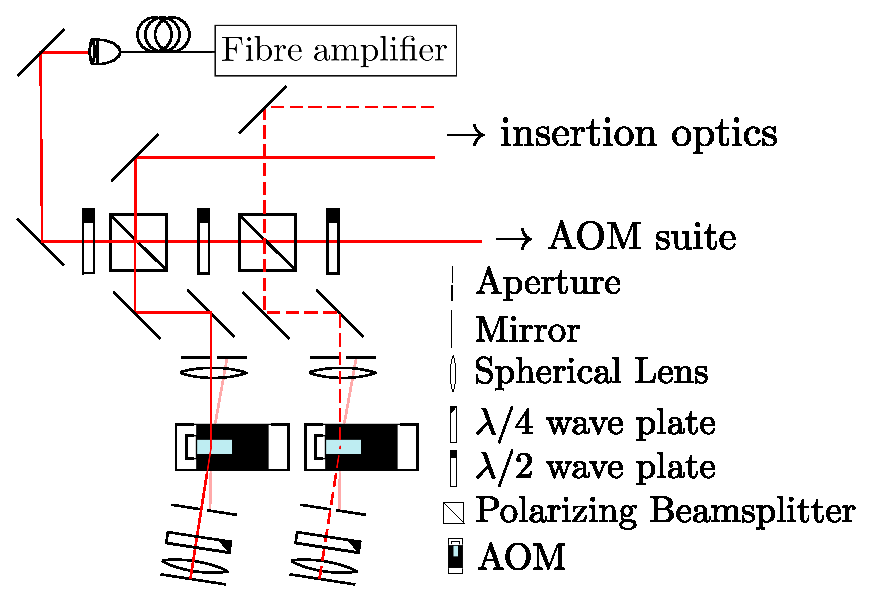
\includegraphics[width=\textwidth]{fig/lattice/distribution_optics}
		  {\fontsize{11}{13}
		  \begin{tabular}{l c c}
		  \hline\hline
		  Beam & Intensity & Detuning \\
		   & $(I_\textrm{sat})$ & ($\Gamma$) \\
		  \hline
		  Collimator &67& -5\\
		  Zeeman &92&-160 \\
		  MOT 1 &87 (Horz.)&-22 \\
		  		&110 (Vert.) & \\
		  Push &110&+3.3 \\
		  MOT 2 &37 (Horz.)& -33\\
		   &140,400 (Vert.)& \\
		  \hline
		  \end{tabular}}
	    \end{minipage}
	\end{figure}

	We had to align the collimator and Zeeman slower beams before the MOT could be built.
	Naturally, having set everything up perfectly the first time, the MOT was nowhere to be found.
	After some further tweaking, we obtained a visual signature of the MOT on the camera, a 1-2 cm diameter smudge in the dark \footnote{We had to switch the room lights off to reduce scattered light in order to spot it.}.
	With some life breathed back into the old machine, it was time for a much larger operation.


\subsection{Vacuum build}

	
	The first stage of the build was to assemble the new science chamber.
	As we were waiting on delivery of the multichannel plates (MCPs) for the final detector, we assembled the second science chamber in order to get the low-velocity intense source (LVIS) operational in the interim.
	The first iteration of this build, prior to the addition of the MOT coils and optics, is shown in Fig. \ref{fig:first_build}.
	The large chamber (manufactured by Kimball physics) features two 8" windows on the flat sides through which the vertical MOT beams and absorption imaging are inserted, and 4.5" windows for insertion of the dipole beams on the top and side opposite the LVIS.
	Several $\frac{1}{2}$" ports are used as feed-throughs for in-vacuum instruments (namely a channel electron multiplier \emph{a.k.a.} channeltron for detecting ions produced by Penning ionization, a non-evaporative getter (NEG) to increase hydrogen adsorption and improve the vacuum, and a Faraday cup on a rotation stage to measure the flux of metastable atoms into the chamber via the LVIS) or covered with windows for optical instruments such as a photodiode to measure fluorescence of the trap.
	The lower assembly includes four-way and six-way crosses (6" flanges each).
	The four-way cross featured a turbomolecular pump (opposite the point of view) which was backed by roughing pump.
	The six-way cross (at the bottom of the stack) featured a residual gas analyser (RGA), whose purpose is described below.
	The entire assembly was put together while supported by four jack stands (one on each horizontal flange of the six-way cross) on a pallet jack.
	The pallet jack could then be wheeled into position and raised to height, and then carefully docked with the back of the gate valve on the MOT.
	The apparatus also featured an old discrete dynode electron multiplier (manufactured by ETP) that was used in early attempts to detect atoms dropped from a magnetic trap, but later stopped working and was thus of no use as a diagnostic for the optical dipole trap.

	The `push' beam was aligned by maximizing the flux from the first MOT into the science chamber as measured by the current on a Faraday cup.
	The sensor was positioned so that it could rotate into the helium beamline from its resting position out of any relevant optical paths.
	The current $I$ (in amps) gives an estimate of the order-of-magnitude flux $\phi_a$ of the atoms by the rule of thumb that $\phi_a\approx I/q$.
	This is an approximate method, but easily suffices for diagnostic purposes.
	Once we obtained a signal that the push beam was reading a current of order 200pA, indicating a flux on the order of 10$^9$ \mhe~atoms per second, we proceeded to assemble the rest of the vacuum system (shown in Fig. \ref{fig:underbelly}) and the MOT optics (detailed in section \ref{sec:new_optics}).
	The strategy was to assemble the MOT and absorption imaging systems to establish the magnetic and dipole traps, then use the ETP electron multiplier to optimize the dipole in the case we were still waiting on the MCP.
	The gate valve below the science chamber meant that we could close off the lower portion of the system and replace a single flange at the bottom of the 24" chamber when installing the MCP-DLD detector stack.
	Thus we would be able to perform the final upgrade without disturbing the MOT optics or breaking vacuum in the MOT chamber, which would be a significant advantage in that it would considerably simplify the necessary bake-out of the vacuum chamber, the subject of the next section.
	

	\begin{figure}
	  \begin{minipage}{0.55\textwidth} %4-8-16
	  \vspace{0pt}
			\includegraphics[width=\textwidth]{fig/lattice/science_chamber_internal}
		   {\begin{flushright}\caption{Initial build of the new science chamber.
	Right: The science chamber features a Faraday cup,  channeltron, and a NEG for vacuum maintenance.
	The camera was initially used to monitor the first MOT. Later uses of the camera are discussed in sections below.
	A 6" gate valve separates the chamber from a temporary assembly underneath the table.
	Top: Internal view of the chamber, taken the preceding day (after which the channeltron was moved to make room for the mounting plate, see below).}\label{fig:first_build}\end{flushright}}
	  \end{minipage}
	  \hfill
	  \begin{minipage}{0.45\textwidth}
	  \vspace{0pt}
		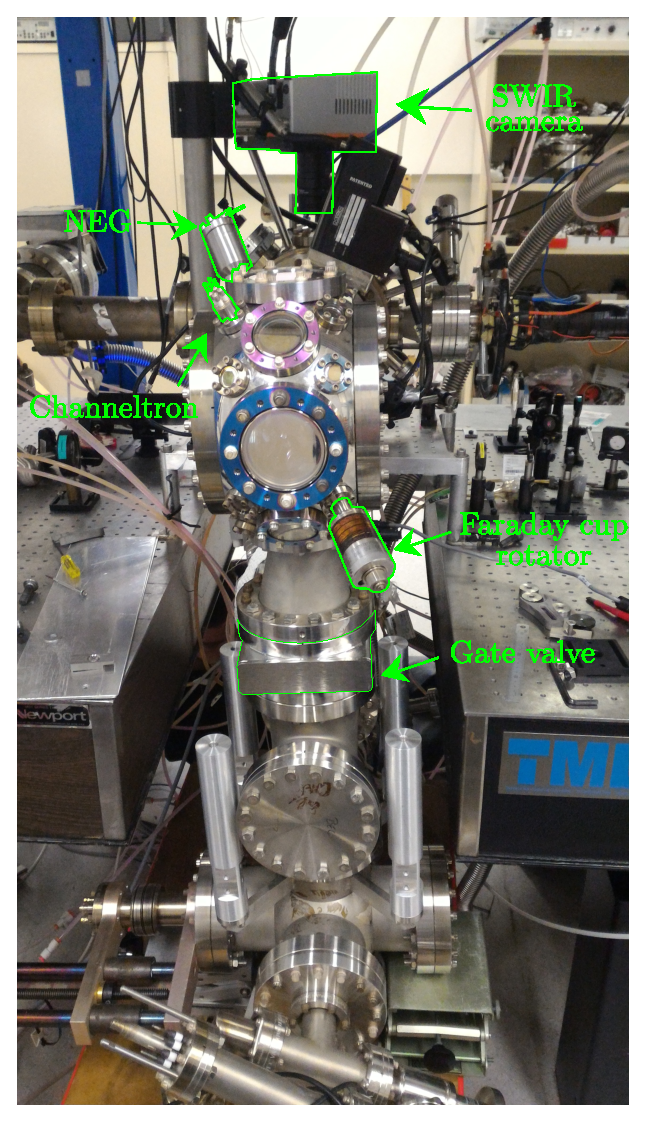
\includegraphics[width=\textwidth]{fig/lattice/science_chamber_profile}  % 5-8-16
	  \end{minipage}
	\end{figure}


	
	
	\begin{figure}
			\centering
		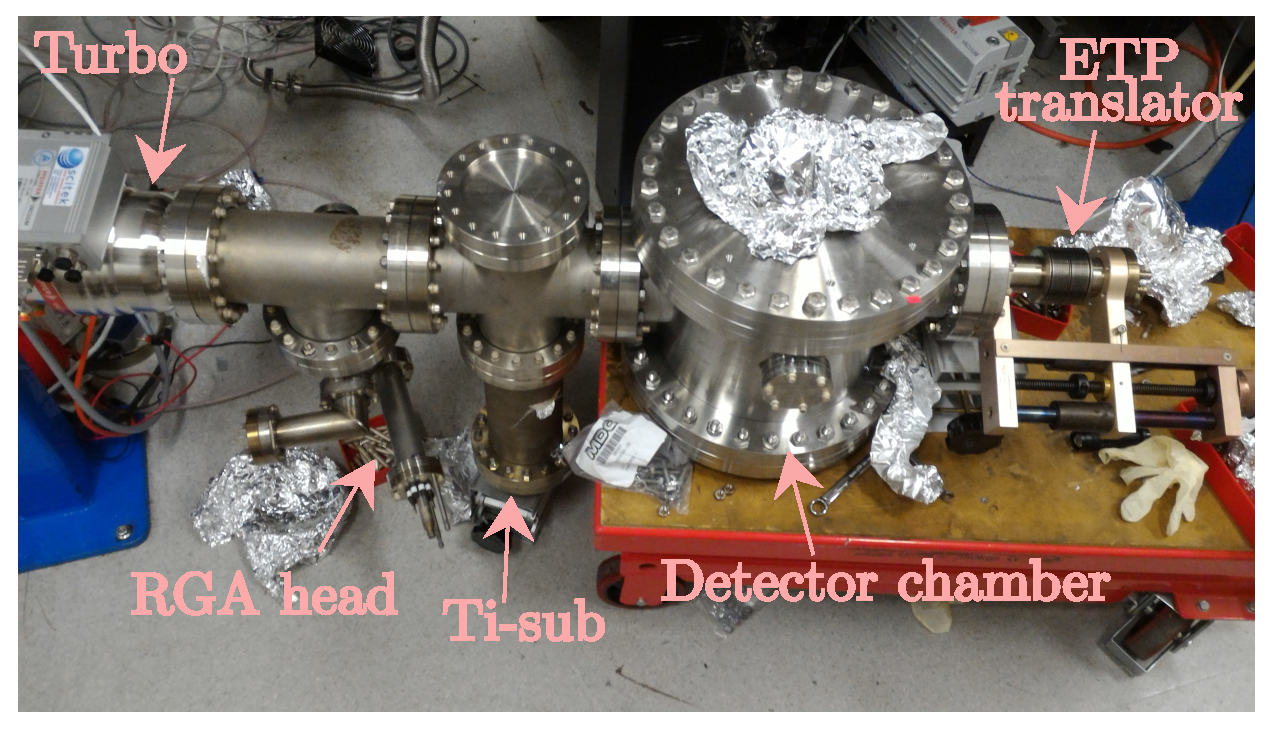
\includegraphics[width=\textwidth]{fig/lattice/detector_level.eps} %15-9-16
		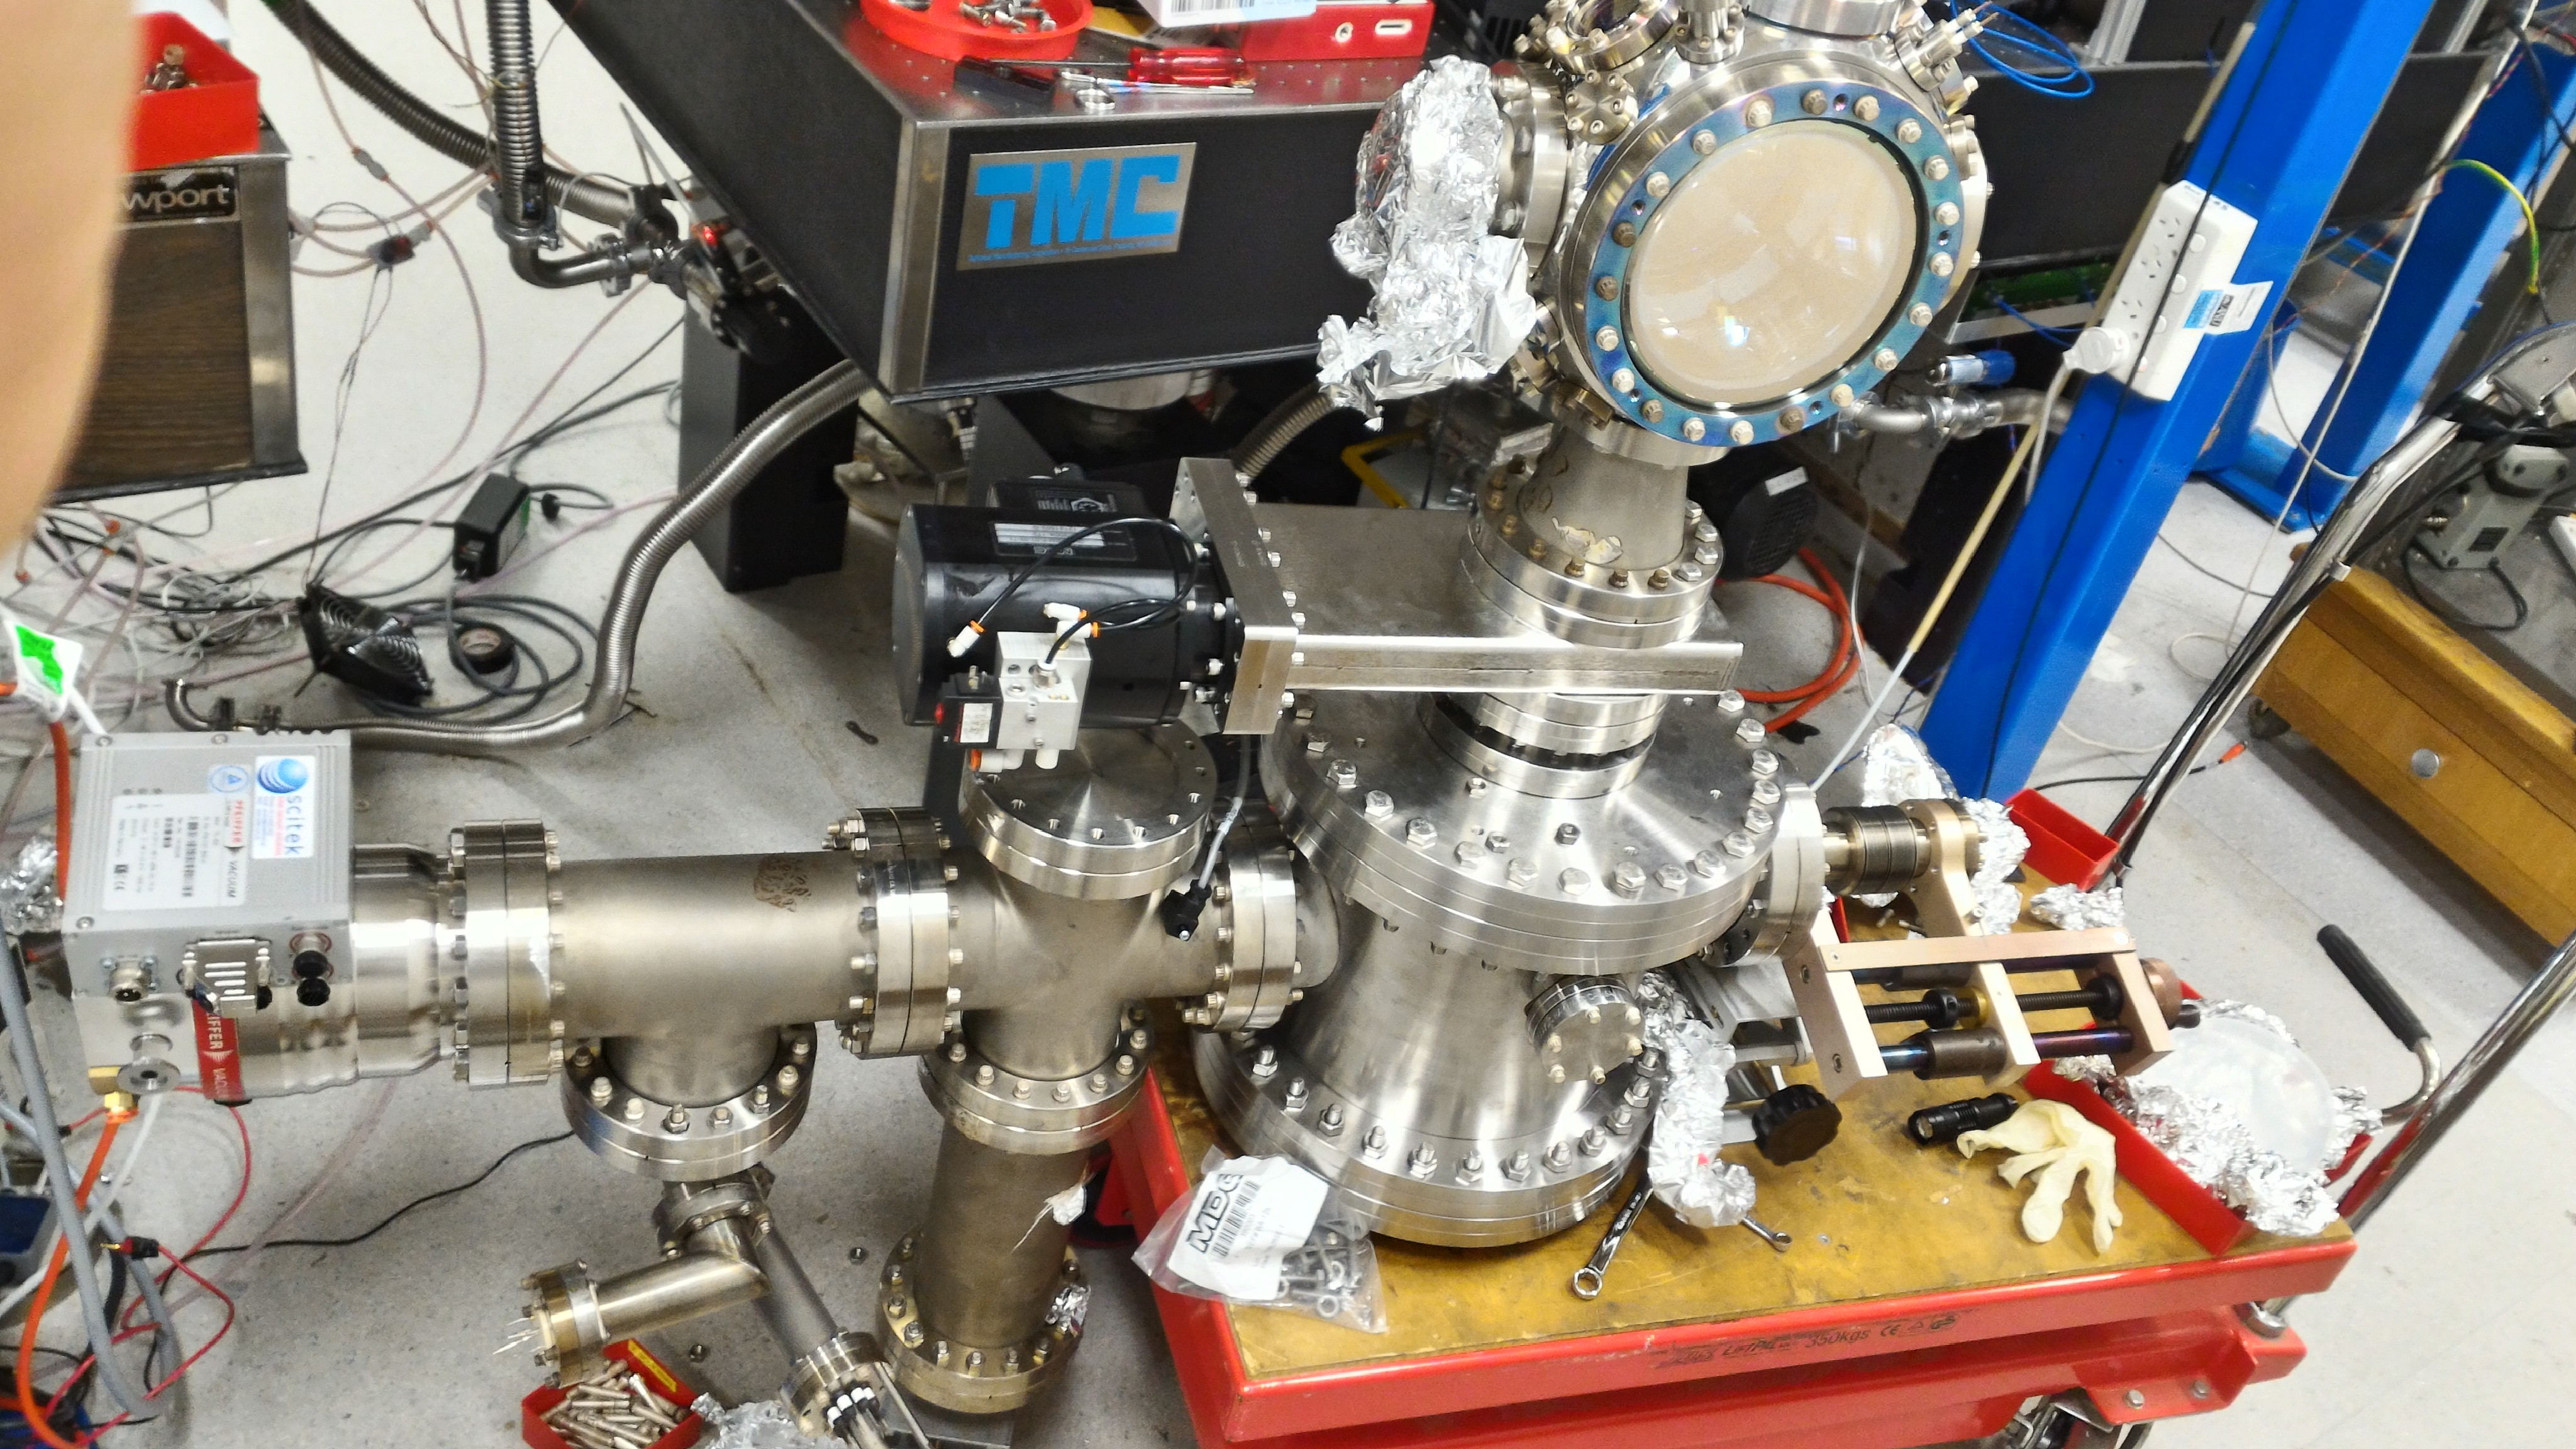
\includegraphics[width=\textwidth]{fig/lattice/full_assembly_20160915} %15-9-16
			\caption{Top: The leviathan-like underbelly of the science chamber resting after assembly on the mobile pallet jack and a smaller hand jack to support the TiSub.
		 Bottom: The science chamber was re-mounted with an intermediate gate valve and then wheeled into place.
		The assembly was stabilized on the blank flange at the bottom of the {24"}-diameter detector chamber, and by being \emph{really} heavy.}
	\label{fig:underbelly}
	\end{figure}

	


	
	\subsubsection{Improving vacuum conditions}

		As mentioned in chapter \ref{chap:apparatus}, the viability of cold-atom experiments depends on having a good quality vacuum.
		Any background gas molecules will typically have thermal velocities of several hundred m/s, with kinetic energies many orders of magnitude larger than the depth of the trapping potentials.
		Thus an overabundance of background gas can dramatically reduce the lifetime of magnetic and dipole traps, rendering evaporative cooling to degeneracy impossible.
		In the case of helium, there is the added issue of the small atomic mass and possibility of Penning ionization (even in low-momentum collisions) which only exacerbate the issue.
		This lab does not maintain cleanroom conditions outside of the optics tables, so even though care was taken to cover components in new foil when they were not being handled, some environmental pollution would be inevitable.
		Water is a common contaminant, but handling errors can also be a problem, and dust or aerosols can accumulate invisibly on the steel surface.
		All of these contaminants become problems when pumping down to vacuum as the pressure rapidly drops below the vapor pressure of many chemicals that may be stable in atmospheric conditions.
		These surface contaminants may outgas slowly (or be comparatively large) and lead to persistent `virtual leaks' in the chamber.
		The standard remedy is to wrap the machine in highly resistive wires insulated with fibreglass, cover it with aluminium foil to keep heat in, and bake the entire apparatus at around 150 degrees celsius for several days.
		The initial evacuation of the chamber by connecting the turbomolecular pumps was enough to observe a magnetic trap, but would be insufficient to make further progress (see Fig. \ref{fig:lifetime}).



		The higher temperature during the bake increases the outgassing rate and can even liberate some contaminants from the surface, allowing them to be pumped out by the turbomolecular pumps.
		In this process one typically observes a sharp rise in pressure as the chamber heats and the contaminants vaporise, and then a decrease to a lower steady-state pressure as the contaminants cease outgassing and the remnants are evacuated.
		Once the pressure stabilizes, the heater tapes can be turned off, and as the apparatus cools the pressure then settles to a steady-state value.
		An example of this procedure is illustrated in Fig.	\ref{fig:bakeouts}.
		The chemical makeup of gaseous contaminants can be determined using a residual gas analyser (RGA) which are essentially compact mass spectrometers.
		Figure \ref{fig:bakeouts} shows the partial-pressure contributions of gaseous contaminants before the first bake.
		
		Even after baking, the pressure may not be low enough to permit long-lived traps.
		Hydrogen leaching from the surface of the steel chamber can be significant, and even permeate the steel on long enough timescales.
		One means of addressing this is with a titanium sublimation pump (TiSub).
		This is not a pump \emph{per se} but rather a titanium filament.
		A pulsed current of $\approx5$ A (duty cycle approximately 30 seconds on, 60 seconds off) heats the filament and causes titanium to sublimate off the filament and adsorb onto the interior surface of the steel vacuum chamber.
		Hydrogen adsorbs to the titanium surface but not to steel, thus creating a `virtual pump' and driving the pressure further down.


		\begin{figure}
		% 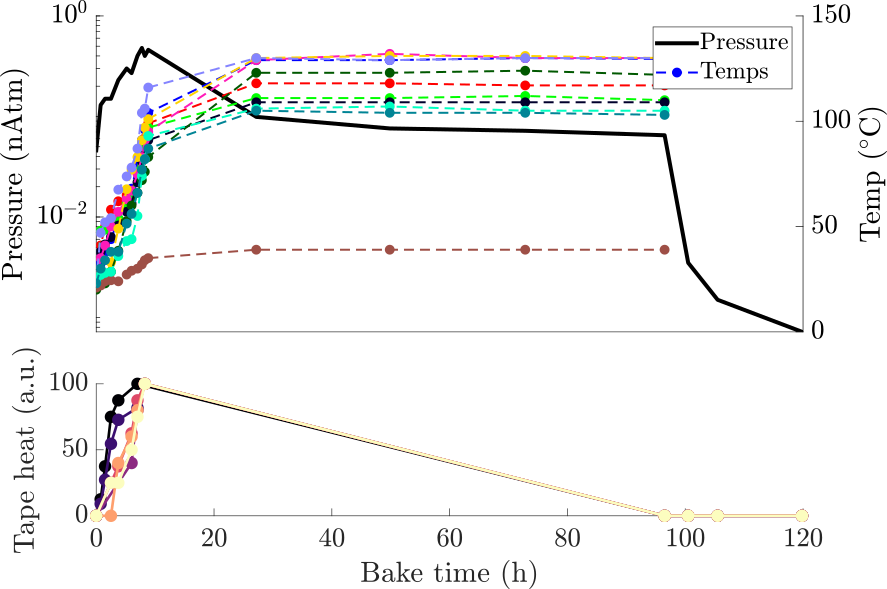
\includegraphics[width=0.5\textwidth]{fig/lattice/mid_december_bake_chart}
		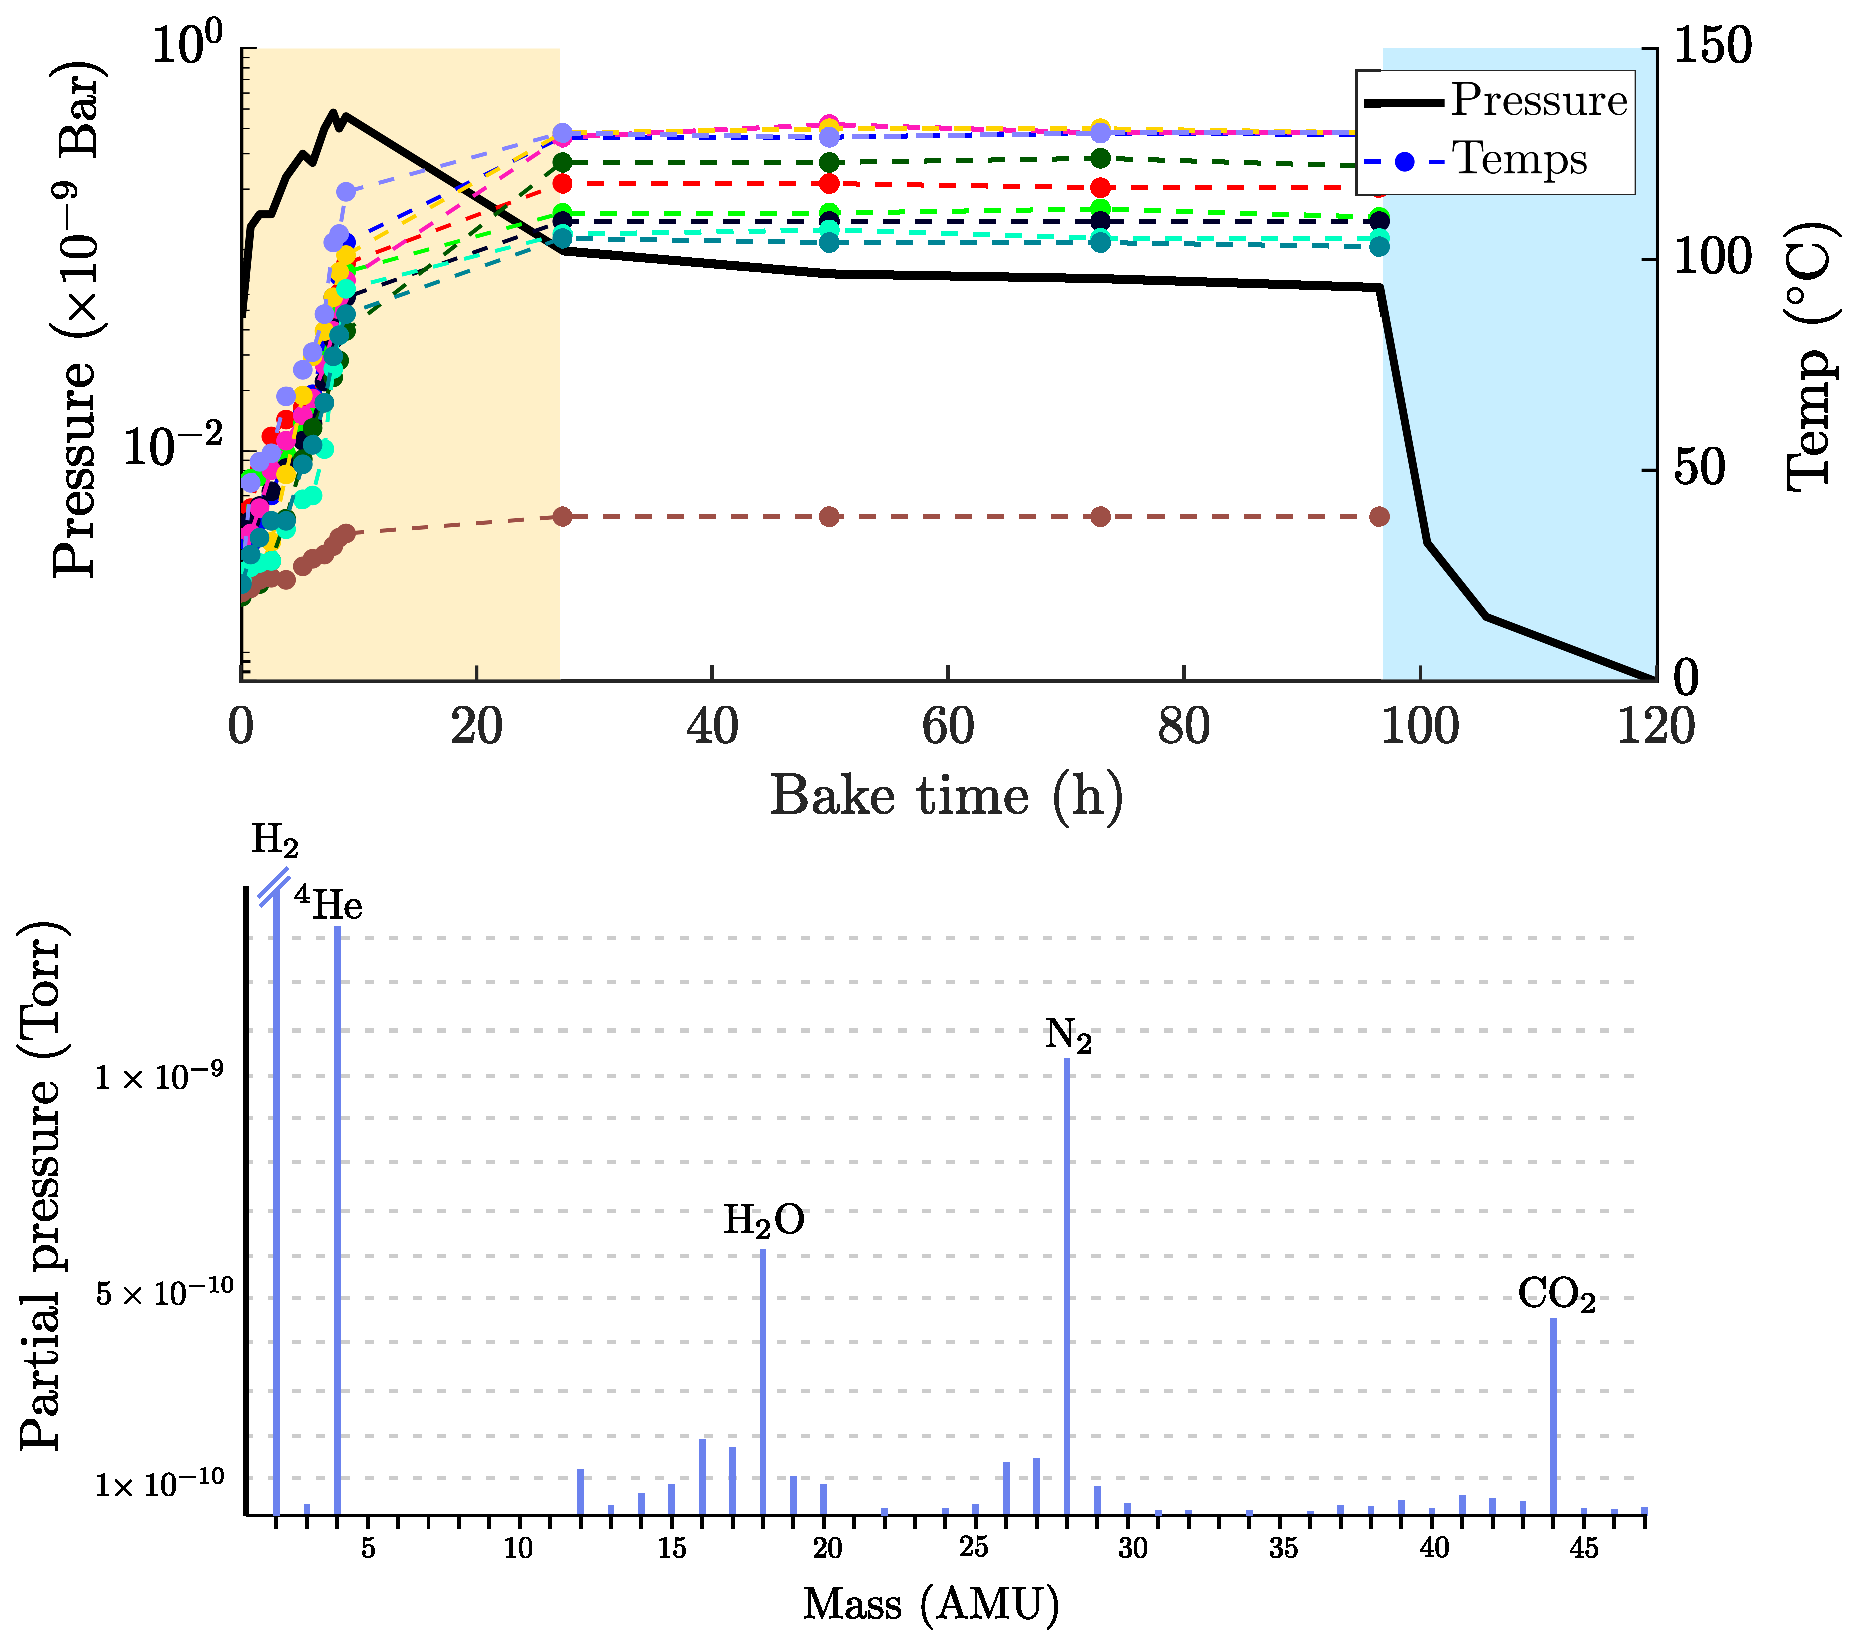
\includegraphics[width=\textwidth]{fig/lattice/RGA_pre_post_bake_nice}
		\caption{Top: The temperature measured by several thermocouples taped to the surface of the vacuum chamber (dots with dashed lines) and the pressure readout from the ion gauge on the science chamber during a bake.
		The heater tapes are supplied with current from variable voltage sources (variacs) which are turned up gradually to ensure even heating when starting the bake (orange region).
		After the tapes are switched off and the insulating foil opened, the steel quickly cools and the vacuum pressure stabilizes (blue region).
		The lower (brown) temperature curve was measured with a thermocouple on the flange connecting the 6" T-piece to the turbo (see Fig. \ref{fig:underbelly}) which was kept cool to avoid excessive heating of the turbo itself. 
		Lines in this figure are to guide the eye, individual measurements are denoted by the solid points.
		Bottom:
		Gas concentrations before the first bake as measured using the residual gas analyser (RGA).}
		% 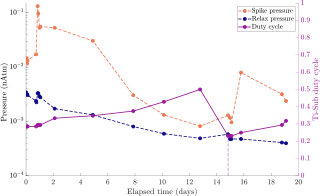
\includegraphics[width=0.9\textwidth]{fig/lattice/tisub_record}
		\label{fig:bakeouts}
		\end{figure}

	Another pressure reduction can be obtained by `getters' which operate in a variety of ways (a TiSub is a kind of hydrogen getter).
	In our machine we used a non-evaporative getter (NEG) in the science chamber.
	The NEG has a highly porous active area which adsorbs hydrogen very strongly.
	This means that they tend to carry in a lot of contaminants and have little remaining active area when first pumping down.
	We cleared the surface of the NEG by passing up to 5 A of current through it.
	Again, the pressure spikes and eventually relaxes up to an hour later, when the current is switched off.
	As shown in Fig \ref{fig:bakeouts}, chamber bakes can improve the chamber pressure by up to three orders of magnitude.
	Afterwards, the TiSub can improve the pressure by a factor of five to ten, and the NEG by a factor of two to five.
		
	The payoff for this multi-stage procedure is the enormous reduction in background pressure that permits long-lived magnetic and (purely) optical traps.
	The lifetime can be quantified by any means that provides a reasonable proxy of the trapped population (the quantity of concern is the relative population at some time later), such as in Fig.	\ref{fig:lifetime}.
	Currently the machine operates at a background pressure below 3$\times10^{-11}$ mTorr (at which point the Ion gauge bottoms out).
		






\subsection{MOT and magnetic trap}
\label{sec:new_optics}

	\begin{figure}
		\includegraphics[width=\textwidth]{fig/lattice/science_chamber_oblique} %4-8-16
		\includegraphics[width=\textwidth]{fig/lattice/science_chamber_optics} %3-5-17
		\caption{The first iteration of the science chamber (in August 2016)  illustrating the coordinate axes used in the lab and the mounting surfaces for the magnetic coils (one of the Anti-Helmholtz (AH) coils was mounted on the back face of the large Kimball chamber). 
		The channeltron is visible on the lower right of the chamber (top), but was moved the next day to make room for the MOT mirror in a similar location in the later image.
		This configuration was used to test vacuum viability and align the LVIS.
		Once the new optic-mounting platform had ben constructed by technician Ross Tranter, we could install the MOT optics (bottom, mounting plate in lower-left quadrant).
		The MOT and imaging beam trajectories are marked, along with the direction of propagation of the LVIS.
		The Faraday cup and NEG are still installed in the lower picture, but the NEG is obscured by the chamber.}
		\label{fig:MOT_optics}
	\end{figure}
	% 1.7e8 atoms loaded at 2.5mK in 1 second, as measured using saturated fluro on an InGaAs PD [26]
	With a good, clean, vacuum and ample optical bench space around the science chamber, the optical components could finally be installed.
	Figure \ref{fig:MOT_optics} shows the enclosing construction around the science chamber that supports a MOT, magnetic trap, and absorption imaging.
	First, the magnetic coils were mounted on the windows to create the anti-Helmoltz field (with axis of symmetry along $x$, parallel to the Zeeman slower) and a bias field directed along the $y$ axis, back along the LVIS.
	The diagonal MOT beams enter through the 2$\frac{3}{4}$" widows on the 45$^\circ$ ports.
	We used the channeltron as a sensor for the presence of a MOT during initial alignment.
	A poorly-aligned MOT (or one with unfavourably set beam parameters) would not have been easily visible by camera or photodiode, but the increase in Penning ionization rate would in principle be controllable by blocking a laser beam and hence provide a fast diagnostic.
	The MOT itself could only be constructed after installing a mounting plate around the base of the vacuum chamber, which was installed after baking the entire new assembly.
	


	\begin{figure}
		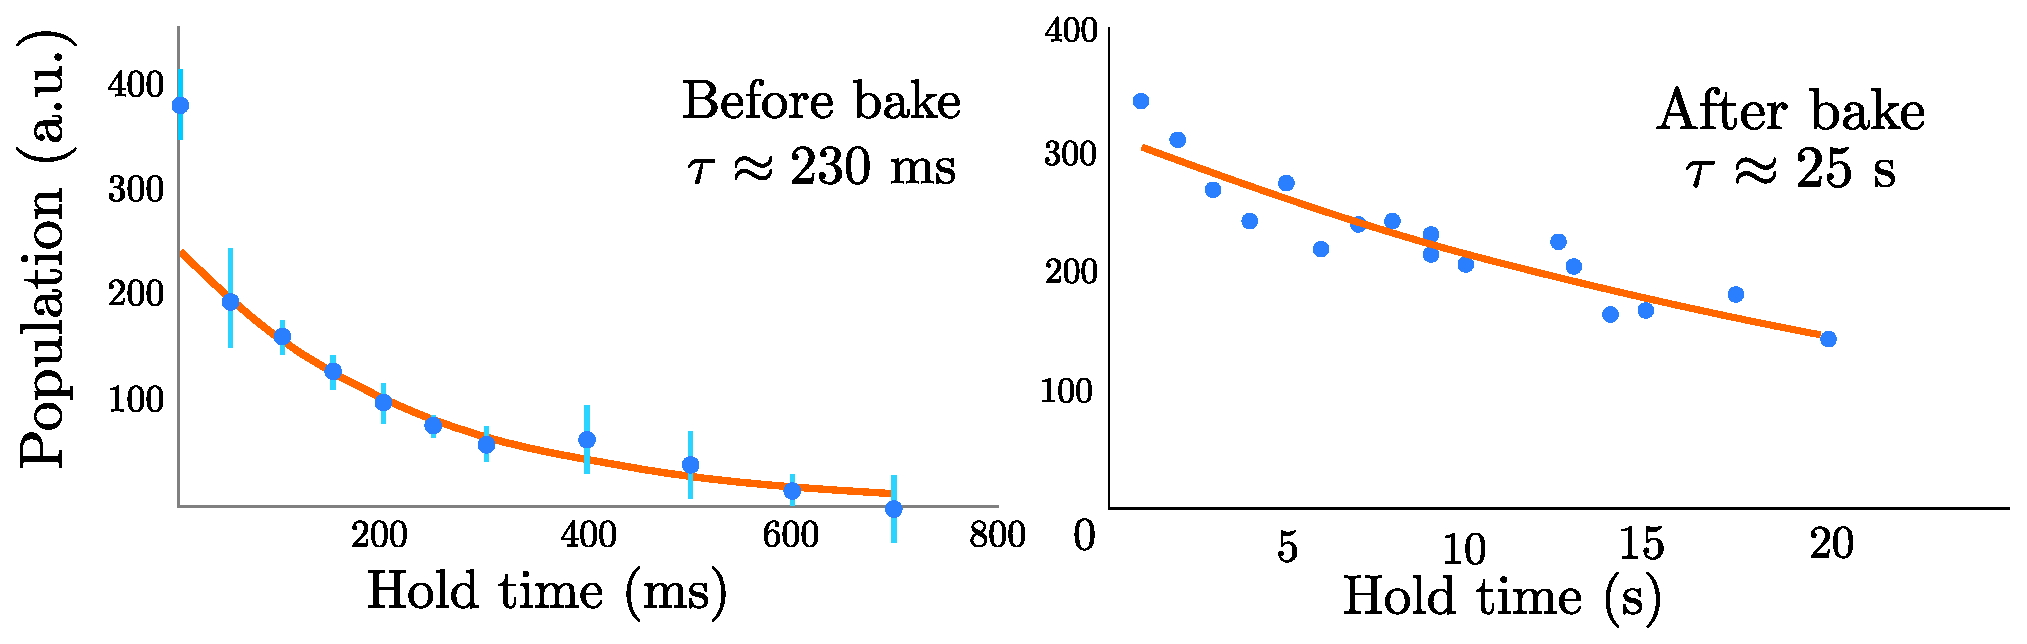
\includegraphics[width=\textwidth]{fig/lattice/trap_lifetimes}
		\caption{Magnetic trap lifetime measurements using before and after baking the new vacuum system. 
		The uncalibrated measurements only show the relative population, due to the measurement method described in section \ref{sec:abs_img}.
		Data points in the left plot are taken from averages of three shots, points on the right plot are single shots.
		The lines in both graphs are exponential fits.}
		\label{fig:lifetime}
	\end{figure}


\subsubsection{Absorption imaging}
\label{sec:abs_img}
		
	Alignment of the dipole trap was eventually made possible by absorption imaging.
	This system is preferred over the MCP-DLD for imaging MOTs and magnetic traps because 
	the clouds can be so wide on the detector that it is impossible to accurately determine the width, thus temperature, of the cloud.
	The analysis can be made more difficult by the potential saturation of the detector at large fluxes.
	A final, albeit lesser, concern is that MOTs and magnetic traps contain thousands of times as many atoms than remain after condensation and so they would shorten the detector's lifespan.
	% This imaging system now provides access to measurements of the temperature, density, atom number, and thus phase space density of a trapped cloud.
	

	\begin{figure}
	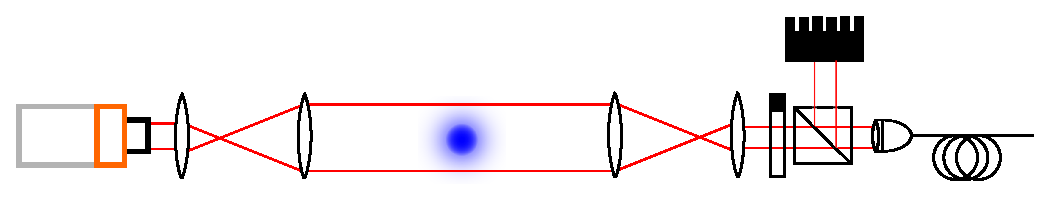
\includegraphics[width=\textwidth]{fig/lattice/abs_img}
	\begin{minipage}{0.44\textwidth}
	\vspace{0pt}
		\caption{ Above: Schematic of the absorption setup as described in the text.
		Adjacent: 
		Example image of the MOT.
		In practise the shot noise on the camera can be significant, and so for visual inspection a smoothing kernel is applied.
		Because of the issues in the text, it is nontrivial to make meaningful inferences about trap properties from in-trap images like these.}
		\label{fig:abs_img}
		\end{minipage}
		\hfill
		\begin{minipage}{0.54\textwidth}
	    \vspace{0pt}
	    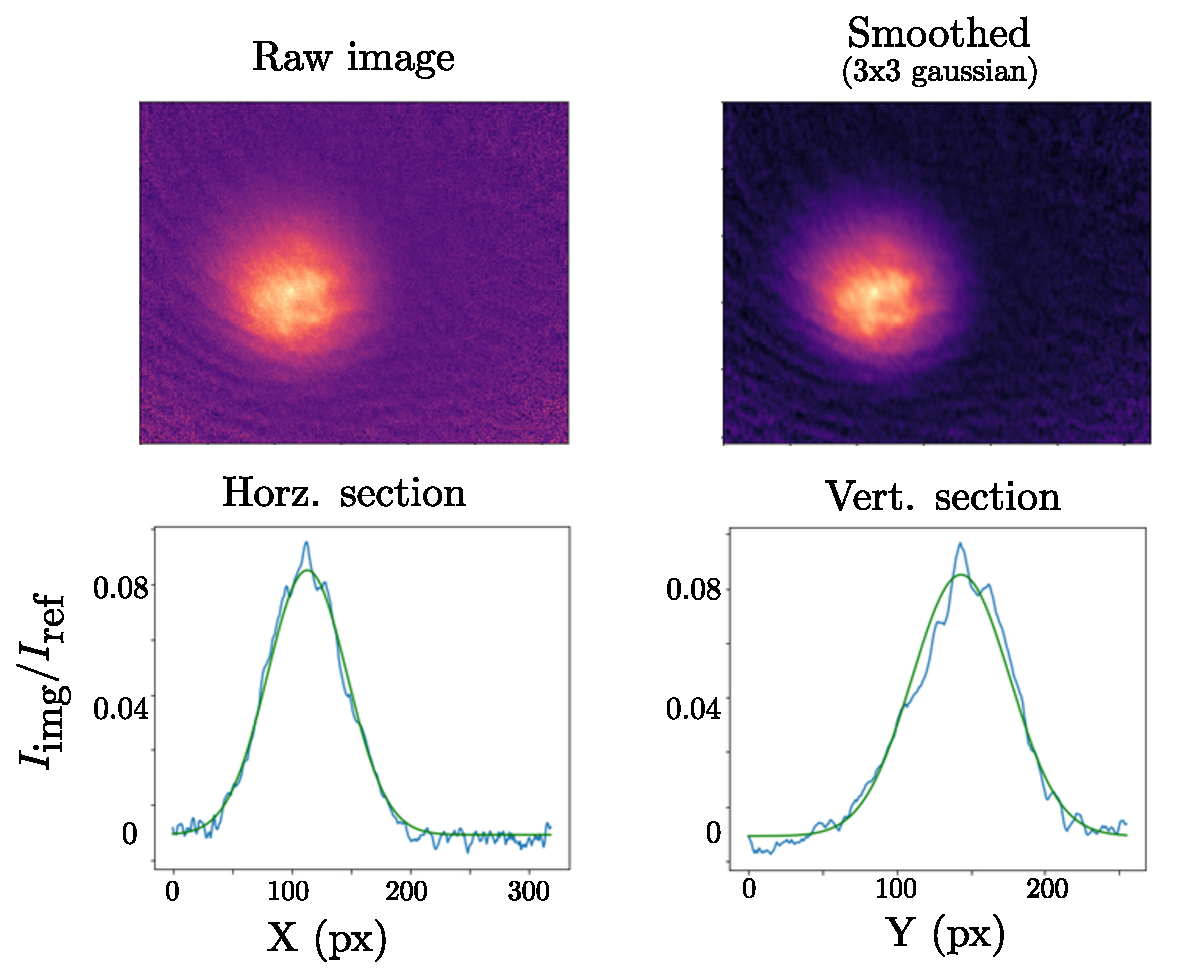
\includegraphics[width=\textwidth]{fig/lattice/20170606_CMOT_img}
	    \end{minipage}
	\end{figure}


	A simple description of absorption imaging is that one `takes a photo of the shadow of the atoms' by illuminating the sample with a collimated laser beam, and then projecting the beam onto a camera (Xenics Bobcat, 256x320 pixel InGaAs sensor, 20 $\mu$m pixel pitch).	
	Detailed discussions of the physical principles and implementations of this technique are presented in \cite{MakingProbingUnderstanding,TychkovThesis}.
	Here we present a simple picture, and an illustration in Fig. \ref{fig:abs_img}.
	A laser tuned close to resonance with the atomic sample is coupled via optic fibre to the absorption imaging setup.
	The light passes through a polarizing beam splitter and then a half-wave plate to fix the polarization, which is useful when imaging in the presence of a bias field\footnote{And indeed the earth's field, which was later found to be strong enough to suppress Penning ionization sufficiently to achieve condensation \cite{Abbas21}.}.
	The beam is then magnified by a 4:1 telescope to a $\approx1$ cm collimated waist and directed at the atomic sample through the vacuum windows.
	The electric field on the exit side of the cloud will have been attenuated by a factor $Ae^{i\phi}$, where the attenuation factor $A=\exp(-\frac{\tilde{n}\sigma_0}{2}\frac{1}{1+\delta^2})$ depends on the column density  $\tilde{n} = \int n(x) dx$ (integrated along the beam axis), the detuning in (half-linewidths) $\delta=2(\omega-\omega_0)/\Gamma$, and the absorption cross-section which is $3\sigma_0\lambda^2/2\pi$ in the two-level approximation \cite{MakingProbingUnderstanding}.
	The phase $\phi$ also depends on the atomic density and detuning from resonance, and is in principle useful for techniques like phase contrast imaging, but is not presently used in this apparatus.

	The camera records an image during the application of the laser light and a second image of identical exposure time after a {$\approx$10 ms delay}\footnote{We found it helpful to ensure that the AOM switched off in the meantime as well, and turned back on for the same cycle time for the second measurement.
	The AOMs can exhibit slow rise-times to their steady state pointing and efficiency due to dissipation of heat into the crystal from the RF drive.
	This was measurable as differences in the light intensity between subsequent images if the AOM was left on between exposures.}.
	By this point the atoms have scattered many photons and left the laser path.
	The second image is used as a reference to compute the integrated absorption at each pixel.
	A light-free image can be used as a `darkfield' to compensate for the camera's inherent noise profile.
	The ratio of (calibrated) pixel intensities in the presence of atoms $I_\textrm{abs}$ to the reference image without atoms $I_\textrm{ref}$ then provides a measure of the squared transmission coefficient,
	\begin{equation}
	A^2(x,y)=\frac{I_\textrm{abs}-I_\textrm{dark}}{I_\textrm{ref}-I_\textrm{dark}}.
	\end{equation}
	The 2D absorption profile can be fitted for purposes of further quantitative analysis. 
	Imaging in-trap is certainly possible and useful for optimizing performance, but it introduces the complication of a spatially-varying magnetic field.
	This means that the transmission coefficient varies due to the Zeeman shift around the trap.
	However, the initial imaging setup had too large a magnification to image the far-field density distribution which is necessary for thermometry.
	This design was shaped by the objective to load atoms into the dipole trap by using absorption imaging as the diagnostic, hence the magnification was chosen such that the MOT would almost fill the frame of the camera sensor.
	Therefore thermometry was not performed using this technique. 
	This was a shortcoming of the first design which was later remedied by upgrading the magnetic coils (see below), thus producing a more tightly-confining field and thus a denser trap.
	For detection and analysis of clouds released from a dipole trap, the lab currently uses the pulses of current across the MCP plates to infer the time-of-flight of atomic detection events \cite{Abbas21}.
	Calibration of the DLD for reconstruction of spatial information is currently underway.

	We could still perform (approximate) population measurements by fitting a Gaussian profile to the images.
	Unfortunately this was not adequately sensitive to measure the lifetime of the magnetic trap.
	After a short decay time it became impossible to get a good fit or even to see the cloud by eye in the absorption images, and thus the long-time behaviour was inaccessible.
	Instead, we released atoms by turning off the magnetic trap and used the number of detection events from the electron multiplier (manufactured by ETP) as a proxy for the population. 
	The current pulses resulting from atoms landing on electron multiplier were passed through a constant fraction discriminator, amplifier, and pulse rate counter which passed into the LabView software.
	The lifetime could then be obtained by an exponential fit to the measured populations over time.
	Measurements of the magnetic trap lifetime before and after the chamber bake are shown in Fig. \ref{fig:lifetime}.


	
	

\subsection{Dipole trap}
	While the main chamber was unworkable during bakeouts, construction could continue on other components of the machine, including the control and distribution systems for the optical dipole beams.
	These beams are generated by a 1550 nm diode laser with a linewidth of $\approx100$ kHz that seeds a 30 W fibre amplifier.
	The high-power beam is split into two AOM arms in a similar manner to the cooling optics described above.
	This configuration is illustrated  in Fig.	\ref{fig:dipole_optics}.
	% Because of the high power and stability demands, the optics were mounted on sturdier posts.
	
	To mitigate against misalignment of the dipole beams, which would eventually need to be overlapped in the focal region within less than 100 $\mu$m, we coupled light from the generation optics to the shaping optics via high-power NKT Photonics photonic crystal fibres to ensure the downstream optics are independent of the alignment upstream.
	Each AOM was driven at a fixed frequency by an amplified voltage-controlled oscillator, but the drive power was set in closed-loop configuration (in contrast to the cooling optics) to mitigate against heating the trap through intensity fluctuations.
	The voltage from a post-fibre photodiode was returned to a PID controller whose set point was determined by an arbitrary waveform generator pre-loaded with user defined waveforms and triggered by the main DAQ system.
	After losses in AOM transmission efficiency and fibre coupling losses, the maximum achievable (total) efficiency of each arm was about 30\% (defined as the ratio of power delivered into the chamber over the input power to the respective AOM).
	While I was working in the lab, the beam powers were roughly equal, but in the interim the dipole system has been redesigned, as discussed in \cite{Abbas21}.

	
	
	\begin{figure}
		\centering
		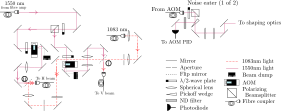
\includegraphics[width=\textwidth]{fig/lattice/dipole_optics}
		\caption{Schematic of the 1550 nm optics used to generate and control the dipole trap beams in the lattice machine.
		The AOMs are used for amplitude control and fast switching, and to run the dipole beams at slightly different frequencies to avoid mutual interference.
		They are driven by dedicated PID controls set in configurable sequences with the arbitrary-waveform generators.
		The beams then focus into an optical fibre which transports the beam to the shaping optics (example on top right).
		Initial alignment of the dipole beams is achieved one beam at a time by inserting one of the removable mirrors (marked (i) and (ii)) and coupling resonant 1083nm light into the fibre.}
		\label{fig:dipole_optics}
	\end{figure}
	

	It is generally desirable to operate far-red-detuned dipole traps at very high intensities to create deeper traps (recall the ground-state shift scales with the intensity $I$, c.f. chapter \ref{chap:theory}).
	Deeper optical dipole traps can contain more atoms at a given temperature by virtue of trapping over a larger range of particle momenta, and so greater laser intensity is generally a good thing.
	It is true that spontaneous off-resonant scattering rates increase (approximately linearly) with intensity, but this can be remedied by detuning further (the scattering rate falls off with $\Delta^2$).
	Therefore one can obtain better loading efficiencies by using brighter beams.
	The purpose of the shaping optics are thus to shape the profile of the beam such that it reaches a tight focus.
	In order to achieve this, given the non-collimated laser profile emitted from the fibres, we first had to determine the profile of the beam, and then determine an arrangement of lenses to shape the beam to a tight focus at the desired trap location.
	The procedure we used to construct the shaping and insertion optics are discussed here.
	We aligned the beam output from the fibre parallel to a 1m-long rail which would be used to mount the lenses.
	We measured the profiles (at low power) by taking images with an InGaAs camera and fitting the output images with 2D gaussian profiles.
	A constrained two-dimensional Gaussian fit yields the waists $\sigma_x$ and $\sigma_y$ along the frame axes.

	A collection of measurements of the waists at positions $z_i$ along the rail can be fitted by the expression $w(z) = w(0)\sqrt{1 + (z/z_R)^2}$ for the waist of a Gaussian beam.
	In the preceding expression, $w(z)$ is the beam waist at distance $z$ from the focus and $z_R=\pi w(0)^2n/\lambda$ is the Rayleigh range (in terms of the laser wavelength $\lambda$ and refractive index $n$).
	We can then calculate the complex beam parameter $q(z) = z + i z_R$ and propagate it backward to determine the spot size and radius of curvature at the beginning of the rail.
	We used these values as input to a home-coded optical simulator which predicts the beam waist at a position $z$ after the beam propagates through a user-defined set of lenses and total optical path length.
	An example of such a simulated beam profile is shown in Fig. \ref{fig:profiling}.
	In reality some manual adjustment is necessary.
	The focus was finessed by deflecting the beam along a path of equal length to the distance to the desired trap centre and focusing the beam with respect to a camera at that position.

	\begin{figure}
	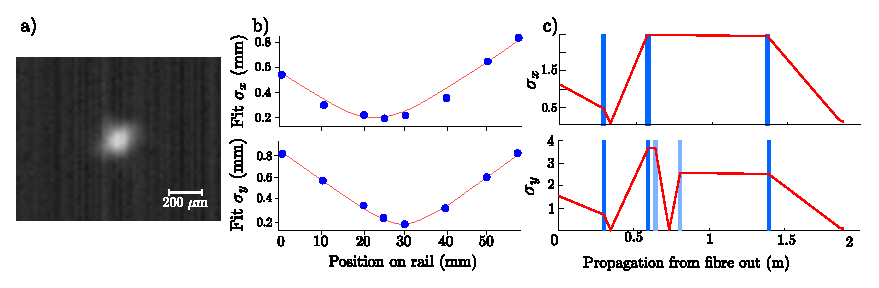
\includegraphics[width=\textwidth]{fig/lattice/dipole_profle_combo}
	\caption{a) Image taken from the InGaAs camera near the focus of a dipole beam.
	b) Beam waists along the rail as obtained from two-dimensional Gaussian fits to the images.
	c) Forward-propagation simulation of the beam waists which was designed to reshape the profiles.
	Cylindrical lenses only act on one of the axes, and are shown in a lighter blue.
	This iterative process produced the image on the left, with waist sizes 130 $\mu$m and 124 $\mu$m.}
	\label{fig:profiling}
	\end{figure}



\subsubsection{Dipole trap}
\label{sec:dipole_trap}

	The dipole beams were first aligned to overlap with the magnetic trap by piping resonant light (at 1083 nm) through the dipole beam delivery fibres instead of 1550 nm.
	To do this, we redirected a few mW of light from the absorption imaging optics using a beamsplitter, passed it through an attenuator, and inserted it into the dipole optics via removable mirrors as illustrated in Fig.	\ref{fig:dipole_optics}.
	The endgame strategy was to achieve BEC by evaporative cooling in an optical dipole trap composed of two beams intersecting at right angles.
	Given total efficiencies of about 30\% through the dipole optics, we could deliver about 5W of power through each beam.
	With each beam focused to a waist of order 100 $\mu$m, the peak intensity of each beam would be $I_0 = 2P/\pi w_x w_y \approx 3.5\times10^9$ mW cm$^{-2}$, and combine to give a dipole trap about 70 $\mu$K deep.
	This highlights the need for very cold magnetic traps (and tightly-focused dipole beams) to ensure many atoms have sufficiently low energy to remain in the dipole trap.
	One also desires a tightly-confined magnetic trap to ensure good spatial overlap of the magnetic trap with the brightest parts of the dipole beam.
	Furthermore, the rate of elastic collisions between trapped atoms increases with tighter traps, which permits more efficient evaporative cooling \cite{Ketterle96}, underscoring the need for tight traps.
	Several iterations of magnetic field configurations and RF ramps were tried during the build but no significant improvement in loading efficiency (based on absorption-imaging measurements) was obtained.
	Due to the aforementioned issues with time-of-flight imaging given the small field of view, the challenges of in-trap imaging, and the low loading efficiency of the dipole trap, precise thermometry was not yet possible.  
	In the end, a key step forward was to install in-vacuum coils (at no small expense of effort) after I had left the lab.
	Details about the present trapping methods are presented in \cite{Abbas21}.
	This includes several re-assemblies of the optics and a change in the dipole trap configuration (namely switching to a second horizontal beam rather than a vertical beam as the upper flange of the Kimball chamber now hosts the coil feed-throughs including their cooling water).
	


	\begin{figure}
		\begin{minipage}{0.43\textwidth}
		\vspace{0cm}
		\caption{The $y$-axis dipole passes through a final focusing lens (lower middle) and is lifted by sturdy optics mounted to a heavy post.
	The upper mirror dials can be remotely controlled, using piezo-driven stepper motors, for precision alignment.
	The camera and refocusing optics for the absorption imaging system are just outside the left of the frame.}
		\label{fig:lifetime}
		\end{minipage}
		\hfill
		\begin{minipage}{0.55\textwidth}
		\vspace{0cm}
		\includegraphics[width=\textwidth]{fig/lattice/dipole_insertion_mirror} %20-11-17
		\end{minipage}
	\end{figure}


	
	However, the basic operation of the dipole is unchanged, including the alignment procedure we discovered, and so is documented here.
	As discussed above, the alignment procedure used resonant light, directed through the dipole fibre into the trap.
	Coarse alignment could be found by supplying light near resonance through the dipole optics after loading a magnetic trap, and optimizing for the destruction of the cloud in response to the beam.
	Alignment could be finessed by reducing the intensity until the cloud recovers, then re-adjusting the beam to hit the centre of the trap and destroy it again.
	The cycle could be repeated until very low intensities were able to destroy the trap.
	Unfortunately we eventually found that there were multiple such optima.
	We determined that these were due to reflections of the beam from the inside of the chamber and scattering back across the trap.
	Afterwards, we acquired the image coincident with the resonant beam (rather than afterward) and found that when the beam intensity was reduced to a mere 4 $\mu$W, the beam appeared to bore a hole through the cloud, as shown in Fig.	\ref{fig:dipole_align}.
	
	\begin{figure}
	\centering
	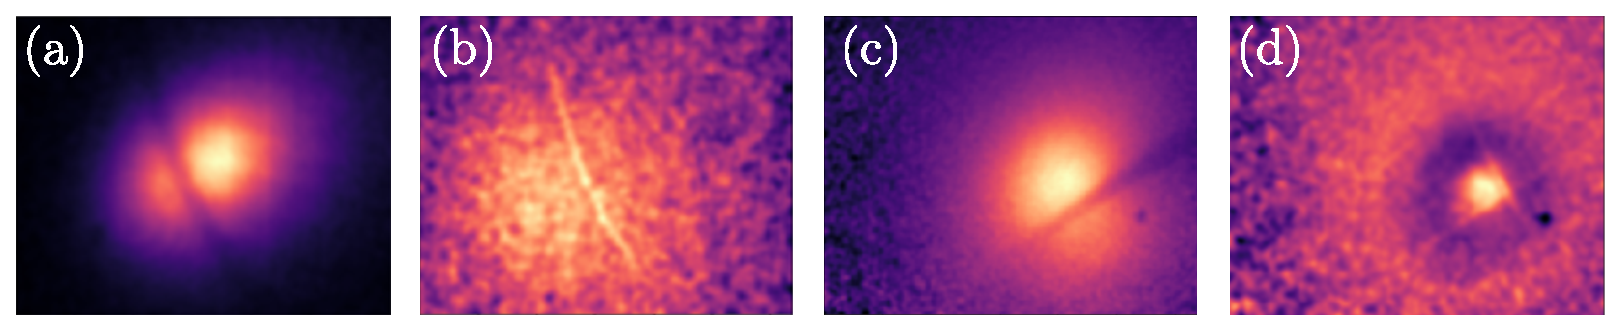
\includegraphics[width=\textwidth]{fig/lattice/dipole_alignment_stages}
		\caption{Stages of dipole beam alignment.
	The first alignment was achieved by passing resonant light through the cloud (a) and triggering the image acquisition (for 10 $\mu$s) at the same time as the resonant pulse.
	After switching to 1550 nm light, the beam deflected slightly due to chromatic aberration in the optics (b) and could then be resolved in averages of 8-10 images. 
	The beam appears to bend in these images because the imaging beam was not aligned with the optical axis of the lenses, which was discovered and corrected using this technique.
	Some time later the vertical dipole was aligned using the same method (c) and so two dipoles could be loaded simultaneously. 
	Finally, an image of the combined magnetic and dipole traps could be taken ((d), average of 10 shots). To obtain this image, a Gaussian fit to the central cloud was subtracted from the image, with a residual halo and bright spot (c.f. the aforementioned issues with in-trap imaging).}
	\label{fig:dipole_align}
	\end{figure}

	After this initial alignment several attempts were made to optimize the dipole loading by adjusting the final lens position, mirror orientation, and experimental control sequences.	
	Matters were made more difficult by several concurrent issues.
	For one, we were \emph{still} waiting for parts for the MCP-DLD detector mount, the ETP electron multiplier had since failed, and the channeltron showed only modest changes in the ionization rate as a function of beam positioning.	
	This left absorption imaging as the sole means of ascertaining the loading efficiency.
	Unfortunately the signal-to-noise was poor and the dipole would only resolve after $\approx 8$ shots.
	At the time the experimental cycle was on the order of 15 seconds, and the long acquistion times were a major obstacle.
	It would eventually be found that the magnetic trap was simply not tight enough.
	The magnetic field gradient would later be improved by upgrade to in-vacuum coils during the tenure of the students who took up the mantle.
	

\section{Progress and outlook}
	


	After my departure, the lab sat motionless for some months as I had been the sole graduate student on the project.
	Later, the \mhe~lattice team was renewed by two PhD students (A. H.	Abbas and X. Meng) and a Masters student (R. S. Patil).
	The team has since achieved a BEC production time of as low as 3.3 seconds, nearly a factor of 2 faster than the prior art \cite{Bouton15} and a factor of 8 faster than the BiQUIC machine.
	The subsequent publication \cite{Abbas21} contains details about the new coils, additional infrastructure and cooling techniques, and characterization techniques.
	The large condensates, containing something on the order of a million atoms, are also competitive with the state-of-the art.
	I take my hat off to the students who picked up the trail where I had left off, and accomplished a goal I'd struggled towards for two years.


	Ahead, the team is faced with the challenge of aligning and optimizing three pairs of lattice beams.
	Once this is accomplished, there is still much ground to cover in exploring the Bose-Hubbard model.
	For instance, the time evolution of the system following a quench or sudden change in dimensionality would be a natural starting point.
	The onset of coherence could be probed via many-particle mometum correlations, extending the work in \cite{Carcy19} into the dynamical regime.	
	Beyond the Bose-Hubbard model, there lies a fork in the road.
	One path leads to the Fermi-Hubbard model by way of further infrastructure upgrades to achieve degenerate $^3$\mhe~in the same machine.
	The expertise gained through the ongoing upgrade of the BiQUIC machine to include $^3$He circulation would be instrumental in this mission.
	The other path is towards the study of the disordered Bose-Hubbard model (also known as the Aubry-Andr\'{e} model), which has been studied in quantum gas microscopes \cite{Rispoli19} but not, so far, with a momentum microscope.
	Theoretical studies predict that momentum-space localization occures in disordered lattices generated by lasers with incommensurate wavelengths \cite{Larcher11}, which is an aspect of localization which has received little attention.
	\vfill
	% \begin{flushright}
	% \singlespacing
	% \emph{``It is not necessary to succeed in order to persevere.\\
	% As long as there is a margin of hope, however narrow, \\
	% we have no choice but to base all our actions on that margin"}\\
	% - Leo Szilard\footnote{\emph{LIFE magazine} volume 51, issue 9, 1961 }\\
	% \end{flushright}
	% \onehalfspacing



	\begingroup
	\begin{flushright}
	
	\singlespacing{\fontsize{12}{12}\selectfont\emph{
	``It might be noted here, for the benefit of those interested in exact solutions, \\
	that there is an alternative formulation of the many-body problem:\\
	How many bodies are required before we have a problem? \\
	G.	E.	Brown points out that this can be answered by a look at history.	\\
	In eighteenth-century Newtonian mechanics,
	the three-body problem was insoluble.\\
	With the birth of general relativity and quantum electrodynamics in 1930,\\ 
	the two- and one-body problems became insoluble.
	And within modern\\
	quantum field theory, the problem of zero bodies (vacuum) is insoluble.\\
	So, if we are out after exact solutions, no bodies at all is already too many!"}\\
	- Richard Mattuck\footnote{R.
	Mattuck, \emph{A Guide to Feynman Diagrams in the Many-Body Problem}, Dover Books on Physics (1992)}
	}
	\end{flushright}
	\onehalfspacing
	\endgroup
	\vspace{1cm}
